% This is "sig-alternate.tex" V2.1 April 2013
% This file should be compiled with V2.5 of "sig-alternate.cls" May 2012
%
% This example file demonstrates the use of the 'sig-alternate.cls'
% V2.5 LaTeX2e document class file. It is for those submitting
% articles to ACM Conference Proceedings WHO DO NOT WISH TO
% STRICTLY ADHERE TO THE SIGS (PUBS-BOARD-ENDORSED) STYLE.
% The 'sig-alternate.cls' file will produce a similar-looking,
% albeit, 'tighter' paper resulting in, invariably, fewer pages.
%
% ----------------------------------------------------------------------------------------------------------------
% This .tex file (and associated .cls V2.5) produces:
%       1) The Permission Statement
%       2) The Conference (location) Info information
%       3) The Copyright Line with ACM data
%       4) NO page numbers
%
% as against the acm_proc_article-sp.cls file which
% DOES NOT produce 1) thru' 3) above.
%
% Using 'sig-alternate.cls' you have control, however, from within
% the source .tex file, over both the CopyrightYear
% (defaulted to 200X) and the ACM Copyright Data
% (defaulted to X-XXXXX-XX-X/XX/XX).
% e.g.
% \CopyrightYear{2007} will cause 2007 to appear in the copyright line.
% \crdata{0-12345-67-8/90/12} will cause 0-12345-67-8/90/12 to appear in the copyright line.
%
% ---------------------------------------------------------------------------------------------------------------
% This .tex source is an example which *does* use
% the .bib file (from which the .bbl file % is produced).
% REMEMBER HOWEVER: After having produced the .bbl file,
% and prior to final submission, you *NEED* to 'insert'
% your .bbl file into your source .tex file so as to provide
% ONE 'self-contained' source file.
%
% ================= IF YOU HAVE QUESTIONS =======================
% Questions regarding the SIGS styles, SIGS policies and
% procedures, Conferences etc. should be sent to
% Adrienne Griscti (griscti@acm.org)
%
% Technical questions _only_ to
% Gerald Murray (murray@hq.acm.org)
% ===============================================================
%
% For tracking purposes - this is V2.0 - May 2012

\RequirePackage{fix-cm}

\documentclass{sig-alternate-05-2015}

\usepackage{graphicx}
\usepackage{epstopdf}
\usepackage{amsmath}
\usepackage{caption}
\usepackage{subcaption}
\usepackage{graphicx}
\usepackage{tikz}
\usepackage{algorithm}
\usepackage{algpseudocode}
\usepackage[font={small}]{caption}
\usepackage[final]{pdfpages}
\usepackage{multirow}
\usepackage{hyperref}

\usepackage{tabularx}
\usepackage{colortbl}
\usepackage{hhline}

\usetikzlibrary{shapes.geometric, arrows}
\tikzstyle{startstop} = [rectangle, rounded corners, minimum width=3cm, minimum height=0.5cm,text centered, draw=black, fill=white]
\tikzstyle{process} = [rectangle, minimum width=3cm, minimum height=1cm,text width=3cm, text centered, draw=black, fill=white]
\tikzstyle{decision} = [circle, minimum size=1cm, text centered, text width=2cm, draw=black, fill=white]
\tikzstyle{io} = [trapezium, trapezium left angle=70, trapezium right angle=110, minimum width=3cm, minimum height=1cm, text centered,text width=3cm, draw=black, fill=white]
\tikzstyle{arrow} = [thick,->,>=stealth]

\usepackage{float}


\begin{document}

% Copyright
\setcopyright{acmcopyright}
%\setcopyright{acmlicensed}
%\setcopyright{rightsretained}
%\setcopyright{usgov}
%\setcopyright{usgovmixed}
%\setcopyright{cagov}
%\setcopyright{cagovmixed}


% DOI
\doi{10.475/123_4}

% ISBN
\isbn{123-4567-24-567/08/06}

%Conference
\conferenceinfo{PLDI '13}{June 16--19, 2013, Seattle, WA, USA}

\acmPrice{\$15.00}

%
% --- Author Metadata here ---
\conferenceinfo{WOODSTOCK}{'97 El Paso, Texas USA}
%\CopyrightYear{2007} % Allows default copyright year (20XX) to be over-ridden - IF NEED BE.
%\crdata{0-12345-67-8/90/01}  % Allows default copyright data (0-89791-88-6/97/05) to be over-ridden - IF NEED BE.
% --- End of Author Metadata ---

\title{Generation of Search-able PDF of the Chemical Equations segmented from Document Images\titlenote{(Produces the permission block, and
copyright information). For use with
SIG-ALTERNATE.CLS. Supported by ACM.}}


\numberofauthors{4} %  in this sample file, there are a *total*
% of EIGHT authors. SIX appear on the 'first-page' (for formatting
% reasons) and the remaining two appear in the \additionalauthors section.
%
\author{
% You can go ahead and credit any number of authors here,
% e.g. one 'row of three' or two rows (consisting of one row of three
% and a second row of one, two or three).
%
% The command \alignauthor (no curly braces needed) should
% precede each author name, affiliation/snail-mail address and
% e-mail address. Additionally, tag each line of
% affiliation/address with \affaddr, and tag the
% e-mail address with \email.
%
% 1st. author
\alignauthor
Prerana Jana\\
       \affaddr{IIEST-Shibpur}\\
       \affaddr{India}\\
       \email{prerana.jana@gmail.com}
% 2nd. author
\alignauthor
Anubhab Majumdar\\
       \affaddr{IIEST-Shibpur}\\
       \affaddr{India}\\
       \email{anubhabmajumdar93\\@gmail.com}
% 3rd. author
\alignauthor Sekhar Mandal\\
       \affaddr{IIEST-Shibpur}\\
       \affaddr{India}\\
       \email{sekhar@cs.iiests.ac.in}
\and  % use '\and' if you need 'another row' of author names
% 4th. author
\alignauthor Bhabatosh Chanda\\
       \affaddr{ISI-Kolkata}\\
       \affaddr{India}\\
       \email{chanda@isical.ac.in}
%% 5th. author
%\alignauthor Sean Fogarty\\
%       \affaddr{NASA Ames Research Center}\\
%       \affaddr{Moffett Field}\\
%       \affaddr{California 94035}\\
%       \email{fogartys@amesres.org}
%% 6th. author
%\alignauthor Charles Palmer\\
%       \affaddr{Palmer Research Laboratories}\\
%       \affaddr{8600 Datapoint Drive}\\
%       \affaddr{San Antonio, Texas 78229}\\
%       \email{cpalmer@prl.com}
}


\maketitle
\begin{abstract}
PDF format of scanned document images is not searchable. OCR tries to remedy this adversity by converting document images into 
editable and searchable data, but it has it's own limitations in presence of equations - both mathematical and chemical. OCR system for mathematical equation  is already a major research area and has provided successful result. However,
chemical equation segmentation has been a less ventured road. In this paper, we present a novel method for automated generation of searchable PDF format of segmented chemical equations from scanned document images by performing chemical symbol recognition and auto-correction of OCR output. We use existing OCR system, pattern recognition technique, contextual data
analysis and a standard \LaTeX\ package to generate the chemical equation in searchable PDF format. The effectiveness of the proposed method is verified through exhaustive testing  on 234 document images. 

\end{abstract}


%
% The code below should be generated by the tool at
% http://dl.acm.org/ccs.cfm
% Please copy and paste the code instead of the example below. 
%
%\begin{CCSXML}
%<ccs2012>
% <concept>
%  <concept_id>10010520.10010553.10010562</concept_id>
%  <concept_desc>Computer systems organization~Embedded systems</concept_desc>
%  <concept_significance>500</concept_significance>
% </concept>
% <concept>
%  <concept_id>10010520.10010575.10010755</concept_id>
%  <concept_desc>Computer systems organization~Redundancy</concept_desc>
%  <concept_significance>300</concept_significance>
% </concept>
% <concept>
%  <concept_id>10010520.10010553.10010554</concept_id>
%  <concept_desc>Computer systems organization~Robotics</concept_desc>
%  <concept_significance>100</concept_significance>
% </concept>
% <concept>
%  <concept_id>10003033.10003083.10003095</concept_id>
%  <concept_desc>Networks~Network reliability</concept_desc>
%  <concept_significance>100</concept_significance>
% </concept>
%</ccs2012>  
%\end{CCSXML}
%
%\ccsdesc[500]{Computer systems organization~Embedded systems}
%\ccsdesc[300]{Computer systems organization~Redundancy}
%\ccsdesc{Computer systems organization~Robotics}
%\ccsdesc[100]{Networks~Network reliability}
%

%
% End generated code
%

%
%  Use this command to print the description
%
\printccsdesc

% We no longer use \terms command
%\terms{Theory}

\keywords{Chemical equations, mathematical symbols, morphological operation.}

%---------------------------------------------------------------------------------------------------%

\section{Introduction}
\label{intro}
Text keywords are used for retrieving  documents from  WWW using search 
engines like Google.
 A large number of documents are being digitized today for the purpose of archival, transmission and browsing. The existing OCR systems show high accuracy in interpreting text portions, but fail to  process other components like graphics, half-tones, chemical and mathematical equations properly.
A few studies \cite{blostein_97},~\cite{chan_00},~\cite{Garain_07} are directed toward math-symbol or math equation recognition assuming that the math-zones are already marked. 
A number of work has been done over the past decade to detect and extract the mathematical equations present in heterogeneous document images. 

  Fateman et al. \cite{fateman_96} proposed a scheme which utilised character size, font information etc.\@ to identify the connected components. Two bags, namely {\em text} and {\em math} are defined. The {\em text }bag is used to  keep   all letters and  numbers; whereas the {\em  math} bag collects punctuation, special symbols, Roman digits, italic letters, lines and dots. Objects in the {\em math} bag are then grouped together according to their spatial proximity. Grouping of items in text bag is   redefined next followed by review and correction to move isolated items to their proper destinations. Math component segmentation is done in \cite{toumit_99} through physical and logical segmentation using spatial characteristics of the math zone as well
  as identifying some math-symbols. The document is then segmented to characters, words, lines and blocks by physical segmentation. The logical segmentation process that follows consists of two steps;
  first the displayed math is detected by identifying their usual center position and in the next step in-line maths is detected by identifying special symbols. 
 
  Kacem et. al. \cite{kacem_01} extracted the equations using fuzzy logic by detecting mathematical  
  operators like '+', '-', etc. Their method was tested on a dataset consisting of 300 expressions and the success rate is about 93\%.   As some of the operators like `+', `-', `(' and `)' do appear in chemical equations as well, it leads to the miss-classification of chemical equations  as mathematical equations reducing the success rate.
A similar method has been proposed in \cite{suzuki_03} to segment    the mathematical expression in printed documents.   The statistical approach taken by Garain \cite{Garain_05} on the corpus of 400 pages to differentiate normal   text lines and lines containing equations/expressions is on the basis of their white spacings which are usually larger in math-equation than the normal text. However, the    chemical equations in the  documents bear the same property. Jin et. al.\cite{jin_03} proposed a similar method to extract displayed formulas using  Parzen classifier.
 
  Drake and Baird \cite{drake_05} came up with a graphical approach; similarly Guo et. al.\cite{guo_07} developed a Gaussian mixture model
  to describe spatial relationships between sub-components of a math expression. 
   Another method to check text style (regular, italic, bold) at the character level has been proposed in \cite{Garain_01}.    Garain \cite{Garain_09} proposed a method to segment the displayed and embedded mathematical formulas from the documents using a     bunch of features. The method is tested on a dataset of 200 images containing 1163 embedded and 1039 displayed expressions    and the success rate is 88.3\% and 97.2\% respectively for embedded and displayed expressions.    A method proposed by Chu and Liu \cite{liu_13} used features based on centroid fluctuation   information on non-homogeneous regions to detect displayed and embedded formulas. 
   
  In a nutshell, in all the above methods emphasis is given only in mathematical equation.  In  eventual segmentation or classification, the chemical equations would automatically be included as a part of mathematical (or other) equations thereby reducing the success rate  of the segmentation and effectiveness of the
subsequent classification, if any. 
 

There are some methods that are used to reconstruct chemical formula from scanned image. They have used chemical datasets. Algorri et al.~\cite{algorri_07,algorri_07a} proposed a system that reconstructs chemical molecules from scanned document. They have used connected component analysis and their own vectorisation algorithm for character recognition. Connected components that are not recognised by the OCR engine, are used to produce a graph of vectors. A rule based approach reconstructs the formula from the vector graph and the character information. 
ChemReader~\cite{park_09} starts with connected component. Alphanumerics are  recognised  using the GOCR open source OCR tool. Graphical components are  identified using Hough transforms, corner detection and other bespoke algorithms.

Jana et al.~\cite{prerana_anubhab_15} proposed a fully automated segmentation and detection technique of chemical equations present in heterogeneous document images. This paper is an extension of their work with some improvements to the original method. We propose a novel automated approach to auto-correct the extracted chemical equations and convert the same into an editable \LaTeX\ file.

The  paper is organized as follows --
Detection and segmentation of chemical equations, auto-correction of the extracted chemical equations and its conversion to PDF form is presented in section~\ref{proposed_algo}. Section~\ref{sc:exp} presents experimental results.
We conclude the paper in section~\ref{sc:con}.


%---------------------------------------------------------------------------------------------------%
 
 

\section{Proposed Work}
\label{proposed_algo}

The proposed
method consists of three distinct steps and they are as follows: (i) Location and extraction displayed chemical equations; (ii) Refining OCR output; and (iii) Converting the extracted chemical equations into search-able PDF format.

\subsection{Location and extraction of
displayed chemical equations}

For this portion of the work, we have largely followed the method proposed in ~\cite{prerana_anubhab_15} with few improvements. 
 
A skew free heterogeneous binary image is the input to the proposed algorithm. 
%The tables and graphics are
%extracted out from the heterogeneous documents using the techniques presented in~\cite{sekhar_06} and~\cite{spc_07} respectively. The rest of
%the document contains normal text lines and displayed equations if any. Our main motivation is to classify chemical and non-chemical equations, we restrict our study to displayed equations (DE) only, as embedded chemical equations are not frequent present in document.

Steps involved for identification of displayed chemical equations are - 
(i) Text line segmentation;
(ii) Word blob formation;
(iii) Operator identification;
(iv) Displayed equation (DE) zone segmentation; and
(v) Classification of extracted DE zone(s);

The details of the aforementioned steps are described in the following subsections.

\subsubsection{Text line segmentation} 
To detect DE zones, text lines have to be segmented first from which the operators are identified to 
 determine whether a text line is a displayed equation or not. We have taken the horizontal projection
 profile of the document page to segment the text line.
%A part of a document page and its horizontal projection profile are shown in Fig.~\ref{H_PROJ}.
%\begin{figure}[h]
%\center\footnotesize 
%\begin{tabular}{|c|}
%\hline
% 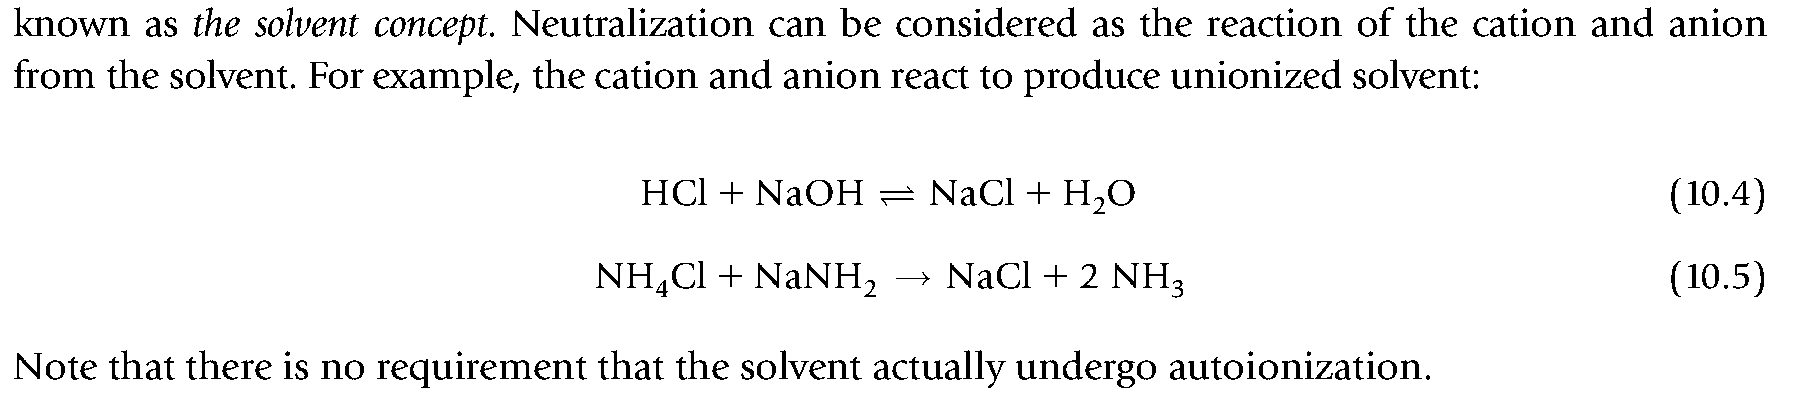
\includegraphics[width=0.45\textwidth]{simage.png} \\ (a) Image\\ 
% \hline
% 
\includegraphics[width=0.45\textwidth]{hProj.png} \\ (b) Horizontal projection \\ 
% \hline
%\end{tabular}
%\caption{ A document page and its horizontal projection profile.}
%\label{H_PROJ} 
%\end{figure} 

\subsubsection{Word blob formation} 
\label{sec:blob}
\begin{figure}[h]
\center\footnotesize 
\begin{tabular}{|c|}
\hline
% 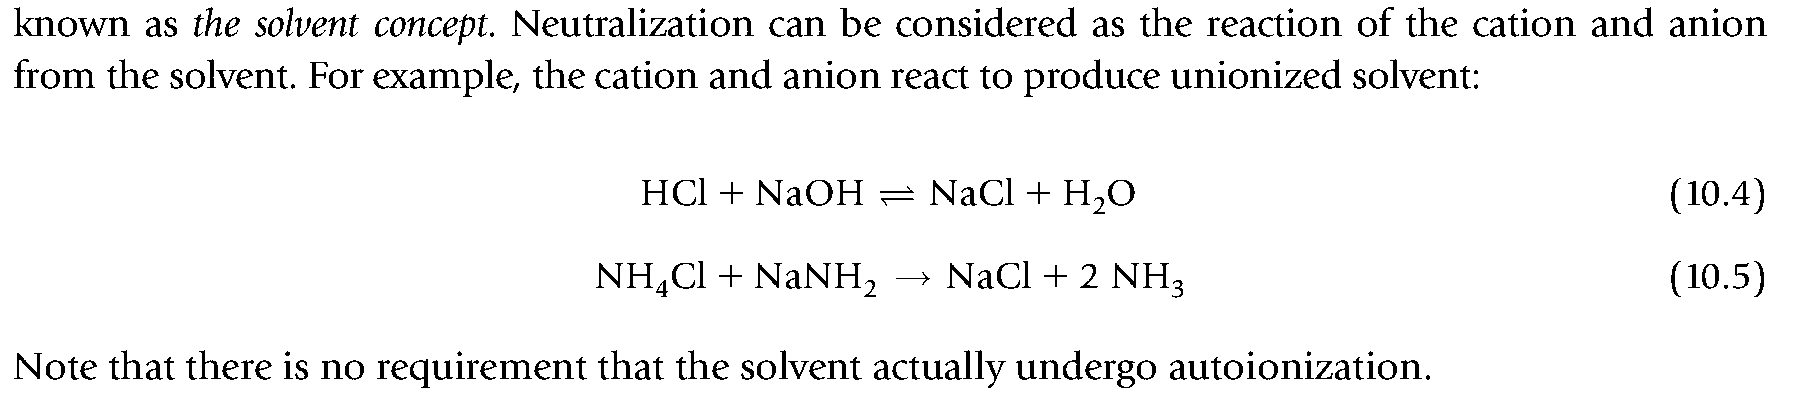
\includegraphics[width=0.45\textwidth]{simage.png} \\ (a) Image \\
%\hline
 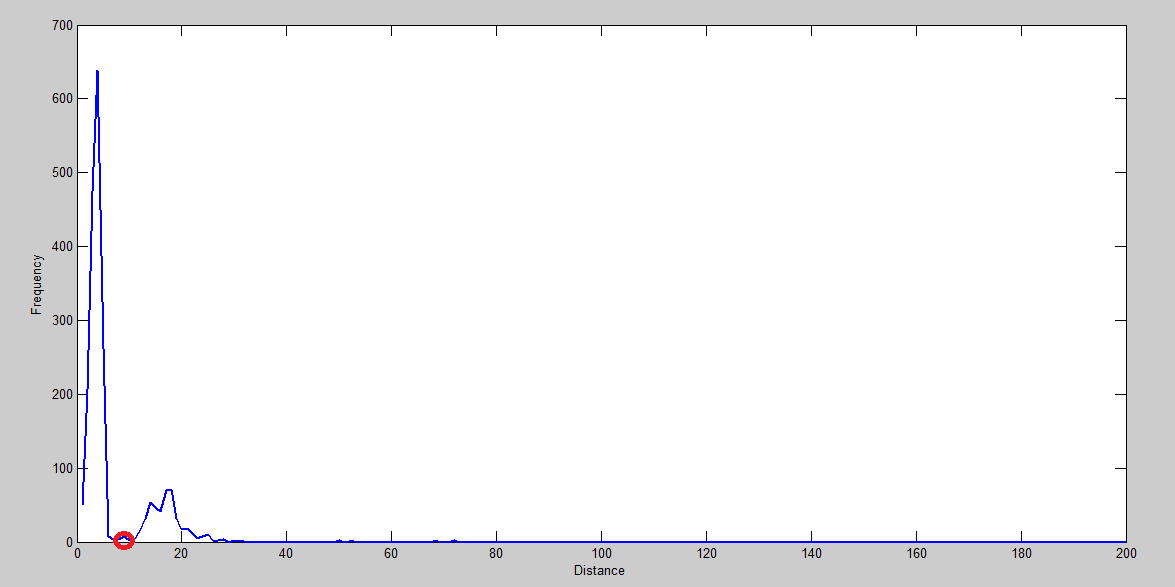
\includegraphics[width=0.3\textwidth]{histogram.png} \\ \\
 \hline
\end{tabular}
\caption{ Distance histogram.}
\label{hist} 
\end{figure} 

This is done by coalescing the characters in a word using morphological closing operation. 
Such character coalescing process depends on the accuracy in detecting the normal
character gap and the gap between the consecutive connected components in that text line.
%The component analysis is done first. 
%
%The mathematical formulation for  blob formation is as follows.
%Consider a binary image $I_{P \times Q}$, which consists of connected
%components $C_k (k=1,2,\ldots ,M)$, as defined in literature.
%Let $C_a$ and $C_b$ be the two consecutive connected
%components in a text line. $L_b$ is the left most x-coordinate of $C_b$ and $R_a$ is the right most x-coordinate of $C_a$. 
%
%Let  $F$ be a function which ensures that the two connected
%components lie in the same text line. $T(C_k)$ and $B(C_k)$ return the topmost y-coordinate and the bottommost y-coordinate of $C_k$.
%Then $F$ may be represented as
%{
%\[F(C_a,C_b)=\left\{ \begin{array}{llc}
%1 & \mbox{if} & (T(C_a)\leq B(C_b)\  AND\  B(C_a)\geq T(C_b)) \\
%0  & \multicolumn{2}{l}{\mbox{otherwise}}
%\end{array} \right. \]
%}
%
%Cluster formation requires information on inter-word gap. 
A histogram with the distribution of distance between
two consecutive characters in the document is plotted.   
%The  distance function, D, obtained from the histogram $H$, is defined for computing the horizontal
%distance between any two consecutive connected components $C_a$ and $C_b$, as shown below
%\[D(C_a,C_b) = L(C_b) - R(C_a)\]
%where $b = \min\limits_x$\{${ L(C_x) - R(C_a)}$\} such that $(F(C_a,C_x) = 1$
%AND $L(C_x)>R(C_a))$.

The distance histogram is a multi-modal histogram. The first peak 
corresponds to the character gaps.
A distance histogram is shown in
Fig.~\ref{hist}.

Our intention is to find out character gaps in running texts of a document page so that we can combine the consecutive characters into a single blob.
 Hence, we consider the upper boundary ($l$) of the first hump as
the length of structuring element. Morphological close operation with a line structuring element of length ($l$) is carried out to form the word blobs. 
%The result of blob formation is shown in Fig.~\ref{BLOB_FORM} for the input image in Fig~\ref{hist}(a).
%\begin{figure}[h]
%\center\footnotesize
%\begin{tabular}{|c|} 
%\hline
%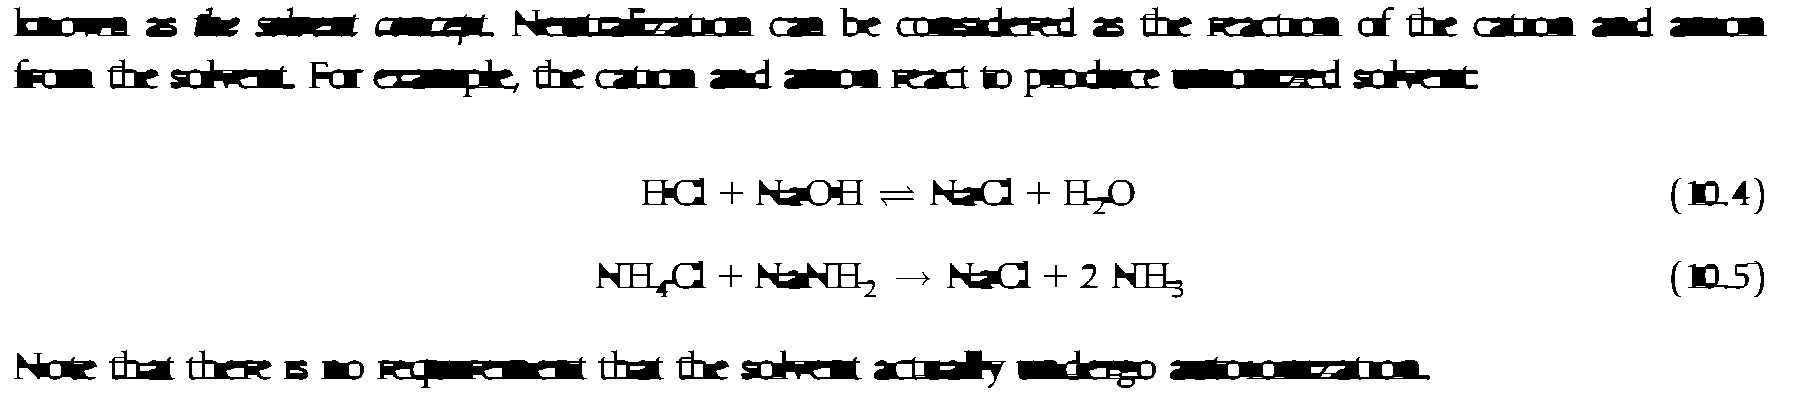
\includegraphics[width=.45\textwidth]{blob.png}\\
%\hline
%\end{tabular}
%\caption{Blob formation of the image shown in Fig.~\ref{hist}(a). } 
%\label{BLOB_FORM} 
%\end{figure}
%\subsubsection{DE zone extraction} 
%\label{DEZONE}



%%%%%%%%%%%%%%   NEW WORK      %%%%%%%%%%%%%%%%%
\subsubsection{Operator detection} 
\label{sec:Op_detection}

In a mathematical or chemical equation, one or more operators are present. These operators signal us the presence of displayed equations in a document. 
%So, we have identified the common \emph{operators} used in chemical and mathematical equations to segment the displayed equations from a text document image.
We have considered the set of \emph{operators} (+, -,  $\rightarrow$, $\leftarrow$, $\leftrightarrow$,  $\rightharpoonup$, $\leftharpoondown$) which are commonly used both in chemical equations as well as mathematical equations to fulfil our aim to identify displayed zones containing chemical or other equations.

After blob formation, small component like dots of \emph{i and j} are eliminated on the basis of area. The region ($R_c$) corresponding to each blob is cropped using its bounding box information from the original image and the number of connected component(s) present in $R_c$ is counted. 
If the number of components is more than 1,
 then that blob is not an operator and is removed from the blob image. 
% This is done because some chemical equations have some reactants/symbols (such as $\Delta$) just on top or bottom of the arrow   
% and in some cases they enter the bounding box of the arrow.  
% Thus if we extract only single characters from the word blob information 
% we do not get the arrow as it is no longer treated as a single character within its bounding box. 
%The result of this operation is shown in Fig.~\ref{single_char} for the image in Fig.~\ref{BLOB_FORM}. 
%
%\begin{figure}[h]\center\footnotesize
%\begin{tabular}{|c|}\hline
% 
\includegraphics[width=0.45\textwidth]{singleChar.png} \\\hline
% \end{tabular} 
% \caption{Sigle components extracted from the word blobs shown in Fig.~\ref{BLOB_FORM}}
% \label{single_char}
%\end{figure}

The remaining components in the blob image are operators along with some alphanumerics like $‘a’$, $‘A’$, $‘(’$, etc. The logical AND operation is performed between the blob image and the original image. The Euler number of the operators that we have considered is 1  and based on this feature some of the alphanumerics are discarded and the resultant image is denoted by $I_s$

%(Fig.~\ref{after_euler}).
%
%\begin{figure}[h]\center\footnotesize
%\begin{tabular}{|c|}\hline
% 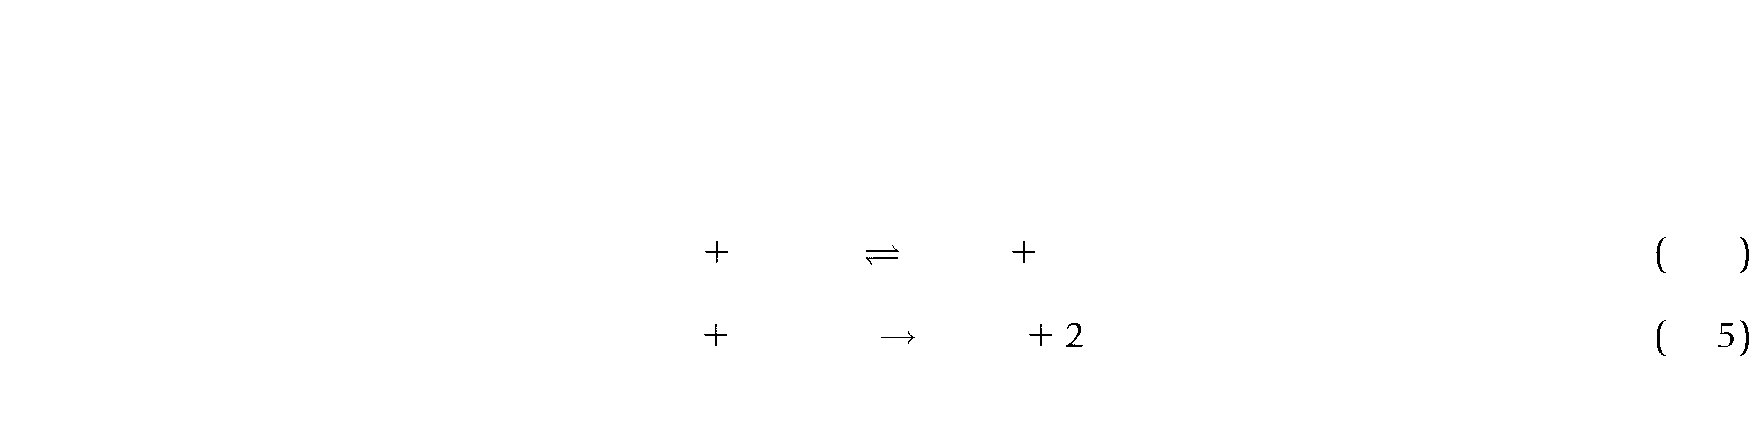
\includegraphics[width=0.45\textwidth]{singleCharafterEuler.png} \\\hline
% \end{tabular} 
% \caption{After removal of alphanumerals based on Euler number from the image shown
%in Fig.~\ref{single_char}}
% \label{after_euler}
%\end{figure}
%


%\begin{figure}[htb]\center\footnotesize
%\begin{tabular}{|c|c|c|}
%\hline
%Operators & horizontal projection & vertical projection\\ \hline
%
\includegraphics[width=0.2in, height=0.2in]{plus.png} &
% 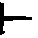
\includegraphics[width=0.2in,height=0.2in ]{plusH.png} & 
%
\includegraphics[width=0.2in,height=0.2in]{plusV.png}\\ \hline
%
\includegraphics[width=0.2in, height=0.02in]{minus.png} &
% 
\includegraphics[width=0.2in,height=0.02in ]{minusH.png} & 
%
\includegraphics[width=0.2in,height=0.02in]{minusV.png}\\ \hline
%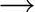
\includegraphics[width=0.2in, height=0.05in]{arrow.png} &
% 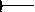
\includegraphics[width=0.2in,height=0.05in ]{arrowH.png} & 
%
\includegraphics[width=0.2in,height=0.05in]{arrowV.png}\\ \hline
%\end{tabular} 
% \caption{Operators and their horizontal and vertical projection profiles}
% \label{h_v_profile}
%\end{figure}

Our next task is identify operator from $I_s$ and for this, we have used a neural network with the following feature set.
% \paragraph{Feature Set:} 
% The simple morphological and topological features are used for operator identification. The features are as follows.
 
\begin{itemize}
 \item Aspect ratio: ($f_a$) of each component
 \item 
 Density: \[f_d   = \frac{\#pixels_o} {\#pixels_b}, \]
 where $\#pixels_o$ denotes the number of object pixels and $\#pixels_b$ denotes area of the bounding box.
 \item The horizontal and vertical projection profiles of each component is obtained.\\
 (i)Spike for horizontal projection profile \[f_{sh} = \frac{\#pixels_{on}}{w} \]
 where $\#pixels_{on}$ denotes the number of on-pixels at the middle of the projection profile and $w$ denotes the width of the profile.\\
 (ii) Spike for vertical projection profile \[f_{sv} = \frac{\#pixels_{on}}{h} \]
 where $\#pixels_{on}$ denotes the number of on-pixels at the middle of the projection profile and $h$ denotes the height of the profile.
 \item Ratio of \[f_{dr}   = \frac{\#pixels_{on}} {\#pixels_{off}}, \]
 where $\#pixels_{on}$ denotes the number of object pixels and $\#pixels_{off}$ denotes the number of background pixels along the diagonal of each component. The ratio is determined for both the right(rd) and left(ld) diagonals.
 \item A binary variable ($f_{open}$): $f_{open} \in \{1, 0\}$.\\
 The value of $f_{open}$ is obtained using morphological opening operation  with a line like structuring element (SE) of length $\frac{w}{2}$, where w is the width of the component.
If the output of the opening operation has a single component, $f_{open}$ is set to 1, else $f_{open}$ is  0.
\item Number of end points ($f_{ep}$): $f_{ep}$ is number of end points of a connected component. This is determined using thinning operation. After thinning each connected component in $I_s$, if a pixel has a single 8-connected neighbor, then that pixel represents  an end point.
 \end{itemize}


Now, [$f_a, f_d, f_{sh}, f_{sv}, f_{dr}^{rd}, f_{dr}^{ld}, f_{open}, f_{ep}$] is the feature vector for classification of operators from 
$I_s$.

%\paragraph{Operator identification:}  

 We classify all single components in $I_s$ into following 4 classes:
\begin{enumerate}
\item Arrows ($\rightarrow$, $\leftarrow$, $\leftrightarrow$,  $\rightharpoonup$, $\leftharpoondown$)

\item Minus (-)

\item Plus (+)

\item Others (~, (, ), etc)

\end{enumerate}

The classification is done using a two-layer feed-forward network with 100 nodes in the hidden layer and sigmoid hidden and softmax output neurons. The network is trained with scaled conjugate gradient back propagation. 

%\begin{figure}[h]\center\footnotesize
%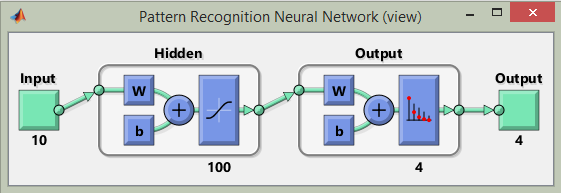
\includegraphics[width=0.45\textwidth]{nn.png}
%\caption{The neural network used to classify single characters from Fig.~\ref{after_euler}}
%\label{nn}
%\end{figure}

We have taken a set of 7046 samples from our image dataset. This set consists of aforesaid operators and other symbol/character.  Out of these 7046 images - 1000 plus, 1000 minus, 1000 arrows and 1000 other single characters are taken for the training set. 

\par The remaining 3046 samples are used for testing the classifier. The accuracy of the network is depicted by the confusion matrix of the test dataset in Table~\ref{table:conMat_final}. The reason for high number of `+' sign in the dataset is because it is the most frequently encountered \emph{operator} as compared to the other operators or single characters. 

 
  
%---------------------------------------------------------------------------------  

%-----------------------------------------------------------------------------------

\begin{table}
\captionof{table}{Results of classifier for identification of \emph{operators}}
\begin{center}
 \begin{tabular}{c c c c c}
  & 1 & 2 & 3 & 4\\
 \hhline{-----}
1 & 319 \cellcolor[gray]{.8}& 0 & 0  & 2\cellcolor[gray]{.95}\\
2 & 0 & 120\cellcolor[gray]{.8}& 0  & 0\\
3 & 0 & 0 & 2267 \cellcolor[gray]{.8}  & 3\cellcolor[gray]{.95}\\
4 & 0 & 0 & 0 & 335 \cellcolor[gray]{.8} \\
\hhline{-----} 
 \end{tabular}
 \end{center}
 \label{table:conMat_final}
 \end{table}

We also need to identify the direction of the arrowhead for its correct representation. The direction of arrowhead is identified by measuring the height of the arrow elements near its two ends. 

%\begin{figure}[h]\center\footnotesize
%\begin{tabular}{|c|}\hline
% 
\includegraphics[width=0.45\textwidth]{operator.png} \\\hline
% \end{tabular} 
% \caption{Extracted operators from the image shown in Fig.~\ref{H_PROJ}(a)}
% \label{operator}
%\end{figure}

To detect `=' or `$\rightleftharpoons$' one extra step is
required. 
For each `-' and `$\rightharpoonup$', a rectangular window of size $l \times l/2$ is
placed below the symbol to check if there is `-' and `$\leftharpoondown$' respectively within
the window; if  present, they are considered to form either  `=' or
`$\rightleftharpoons$' sign. $l$  be the length of the symbol.
The upper boundary of the window  coincides with the lower boundary of the bounding box of each aforesaid symbol.

%\begin{figure}[h]
%\center\footnotesize 
%\begin{tabular}{|c|}
%\hline
% 
\includegraphics[width=0.45\textwidth]{equation.png} \\ (a)\\  
% \hline
% 
\includegraphics[width=0.45\textwidth]{equationOperands.png} \\ (b)\\  
% \hline
%
\includegraphics[width=0.45\textwidth]{equationNumber.png} \\ (c) \\ 
%\hline
%
\includegraphics[width=0.45\textwidth]{hrlsaRemoval.png} \\ (d) \\ 
%\hline 
%\end{tabular}
%\caption{The output of closing operation on portion of an image (a) a part of an image; (b) same part without operators; (c) result of closing operation; (d) after equation number removal.}
%\label{h-rlsa} 
%\end{figure} 

\subsubsection{DE zone exraction} 
\label{sec:DE_zone_extract}

Initially, all the text lines consisting of at least one \emph{operator}
are considered candidate displayed equations (CDE). The
\emph{operators} are separated from CDE. The upper boundary ($u_v$) of
the second hump of distance histogram (Fig.~\ref{hist}) is obtained which
represents the word gaps in the text line. For each CDE zone 
 morphological closing operation with a line structure element of length $u_v$ is
carried out. If the distance between two neighbouring components
is less than $u_v$, it means they belong to a same word and are
merged by closing operation. 
%The output of closing is shown in Fig.~\ref{h-rlsa}.

%Equation numbers are common in the displayed equation zones.
%These numbers have to be removed because 
For each CDE we count the number of \emph{operators} and  other corresponding components in the output of closing operation. If the number of components
$\le$ 2$\times$ number of \emph{operators}, then the CDE is considered
displayed equation; otherwise some embedded formulae/equations
may exist in the line. 

%To eliminate the equation number from the
%output of closing operation, the \emph{operators} are moved to the output of closing operation
%and the component analysis is done. From both ends, distance
%($d$) (Fig. \ref{h-rlsa}(c))
% between the first two consecutive
%components is measured and if $d$ $> 5\times$ $u_v$, then the
%first component from the end is considered the equation number
%and is removed. (Fig. \ref{h-rlsa}(d)).
 
\subsection{Classification of extracted DE zone} 

%Each segment of a displayed equation is divided into three zones; namely
%upper zone, middle zone and lower zone (Fig.~\ref{sub_super}) along vertical direction. To identify the three zones of a DE zone,
%uppermost and lowermost co-ordinates of each connected component
%below the same DE zone are also obtained. The median of
%uppermost coordinate, and median of lowermost co-ordinate of
%such components in DE zone are computed. A virtual horizontal line,
%called the baseline,  separates the middle
%zone and lower zone of DE zone. Similarly, the median of
%uppermost co-ordinate of the components in the DE zone generates
%a horizontal line, called top line, which
%separates the middle and upper zones of the DE zone.
%
%\begin{figure}[h]
%\center\ 
%\begin{tabular}{|c|} 
%\hline
%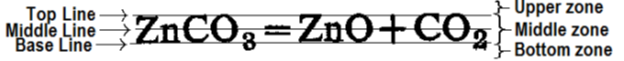
\includegraphics[width=.45\textwidth]{supSub.png}\\
%\hline
%\end{tabular} 
%\caption{Different zones of DE equation}
%\label{sub_super} 
%\end{figure} 
%The subscripts in a DE zone
%belong to lower-half of the middle zone and lower zone whereas
%the superscripts belong to upper zone and upper-half of the
%middle zone. Based on the location of the components in a DE
%zone we have detected the subscripts and superscripts and are
%separated from the DE zone. The operators are also separated
%from DE zone.

The extracted DE zones can be either chemical or other (ex:- mathematical) equations.  
Now, each displayed equation is an input to the inbuilt OCR of MATLAB
R2014a. The OCR returns each DE zone as a text string. We made a
dictionary out of all the elements in the periodic table. An
important observation is that an element always starts with a
capital letter. Using this property, an element can be expressed
by a regular expression [A-Z][a-z]*. It means an element's
symbol starts with an upper case letter and may or may not have
one or more lower case letters (for example $H$, $He$, $Uut$ etc). We have designed a parser to extract the
sub-string matching the regular expression mentioned above with
the following grammar: \begin{center}
\large{
 $start \rightarrow capital.follow$\\ $follow \rightarrow small.follow | \in$\\
$capital \rightarrow A|B| \dots |X|Y|Z$\\  $small \rightarrow
a|b| \dots |x|y|z$\\ }
\end{center} 
%The working principle of the parser is depicted in Fig.~\ref{flow_chart}.
Each of the substring returned
by the parser is matched against the aforesaid dictionary and if
it is a positive match then that substring is considered as a
symbol of the chemical element. Let us consider, the number of
substrings extracted from the OCR output by the parser is {\em
n} and the number of positive matches the aforementioned
dictionary is {\em m}. If m:n ratio is more than a threshold
value $\beta$ then this DE is considered a Chemical Equation.
This threshold ($\beta$) is set to 0.7 experimentally by running the proposed algorithm on  dataset containing 1390 displayed equations. The reason
for the ratio not being 1 are: (i) Limitations of OCR, and (ii)
Touching and broken characters.

%\begin{figure}[h]\center\footnotesize
%\begin{tabular}{|c|}
%\hline
% 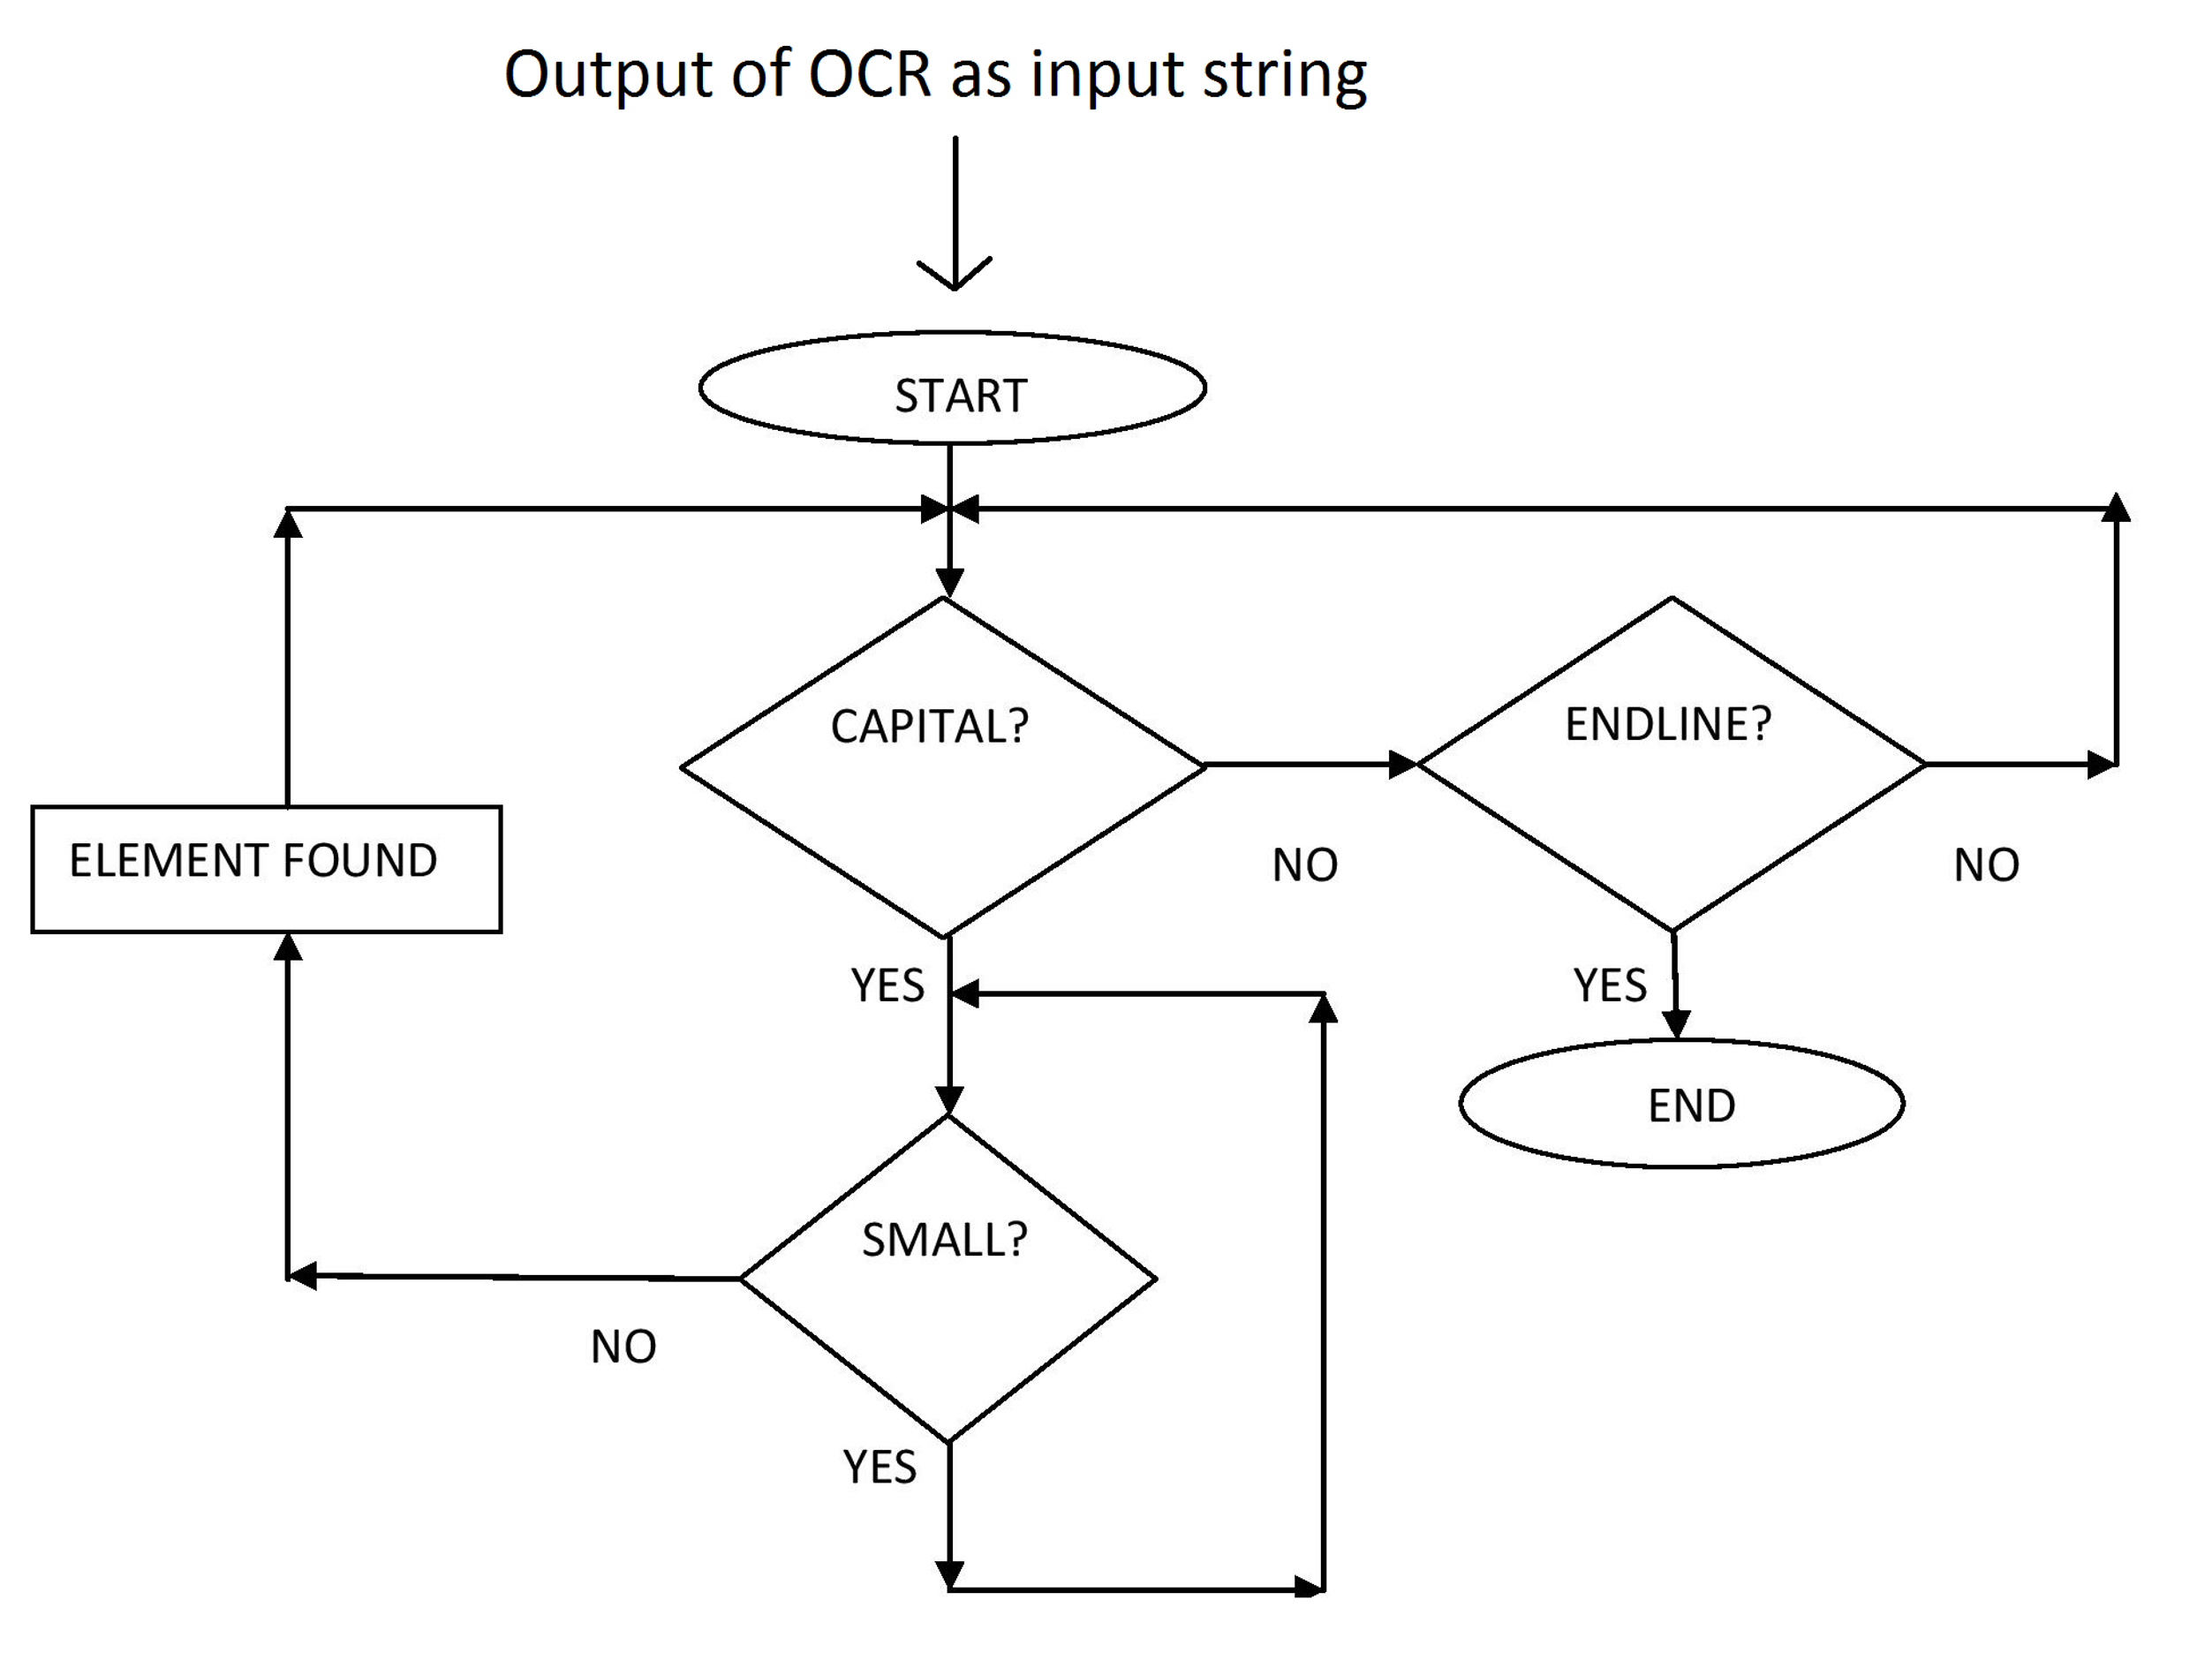
\includegraphics[width=.45\textwidth]{flowchart.png} \\ \hline
% \end{tabular} 
% \caption{Working flow chart of the parser}
% \label{flow_chart}
%\end{figure}



%%%%%%%%%%%%%%%%%%%%%%%%%%%%%%%%%%%%%%%%

\begin{figure}[h]
\center\footnotesize 
\begin{tabular}{|c|}
\hline
 
\includegraphics[width=0.3\textwidth]{arrow_img.png} \\ (a)\\  
 \hline
 
\includegraphics[width=0.3\textwidth]{closed_arrow_img.png} \\ (b)\\  
 \hline

\includegraphics[width=0.3\textwidth]{op_marked.png} \\ (c) \\ 
\hline

\includegraphics[width=0.3\textwidth]{arrow_detected.png} \\ (d) \\ 
\hline 
\end{tabular}
\caption{ Up and down arrow detection (a) A chemical equation; (b) Image after blob formation ; (c) Operators are marked in red; (d) Detected arrow in blue.}
\label{fig:updnar} 
\end{figure} 
The $\uparrow$ and $\downarrow$ are frequently used in chemical equation to represent the state of compounds and  are thus important to detect.
For each identified chemical equation, blob formation is done as discussed in Sec.~\ref{sec:blob}. After  blob formation, we apply component analysis method. Then operators are marked (Fig.~\ref{fig:updnar}(c)) in the blob image, as they are already identified. For each component in blob image (which is not an operator), we  check its immediate left component ($C_l$) and  right component ($C_r$). If none of $C_l$ or $C_r$ is an \emph{operator}, the the component under consideration is an up arrow or a down arrow. Fig.~\ref{fig:updnar}(d) shows the detected up arrow in blue. The identification of the arrowhead is done in the same way as discussed in \emph{operator} detection.


An example of chemical equation segmentation from a sample document image is given in Fig.~\ref{eg}. Fig.~~\ref{eg}(c) shows the output in PDF without any correction.

 

\begin{figure}[]
\center\footnotesize
\begin{tabular}{ |c|}
\hline
 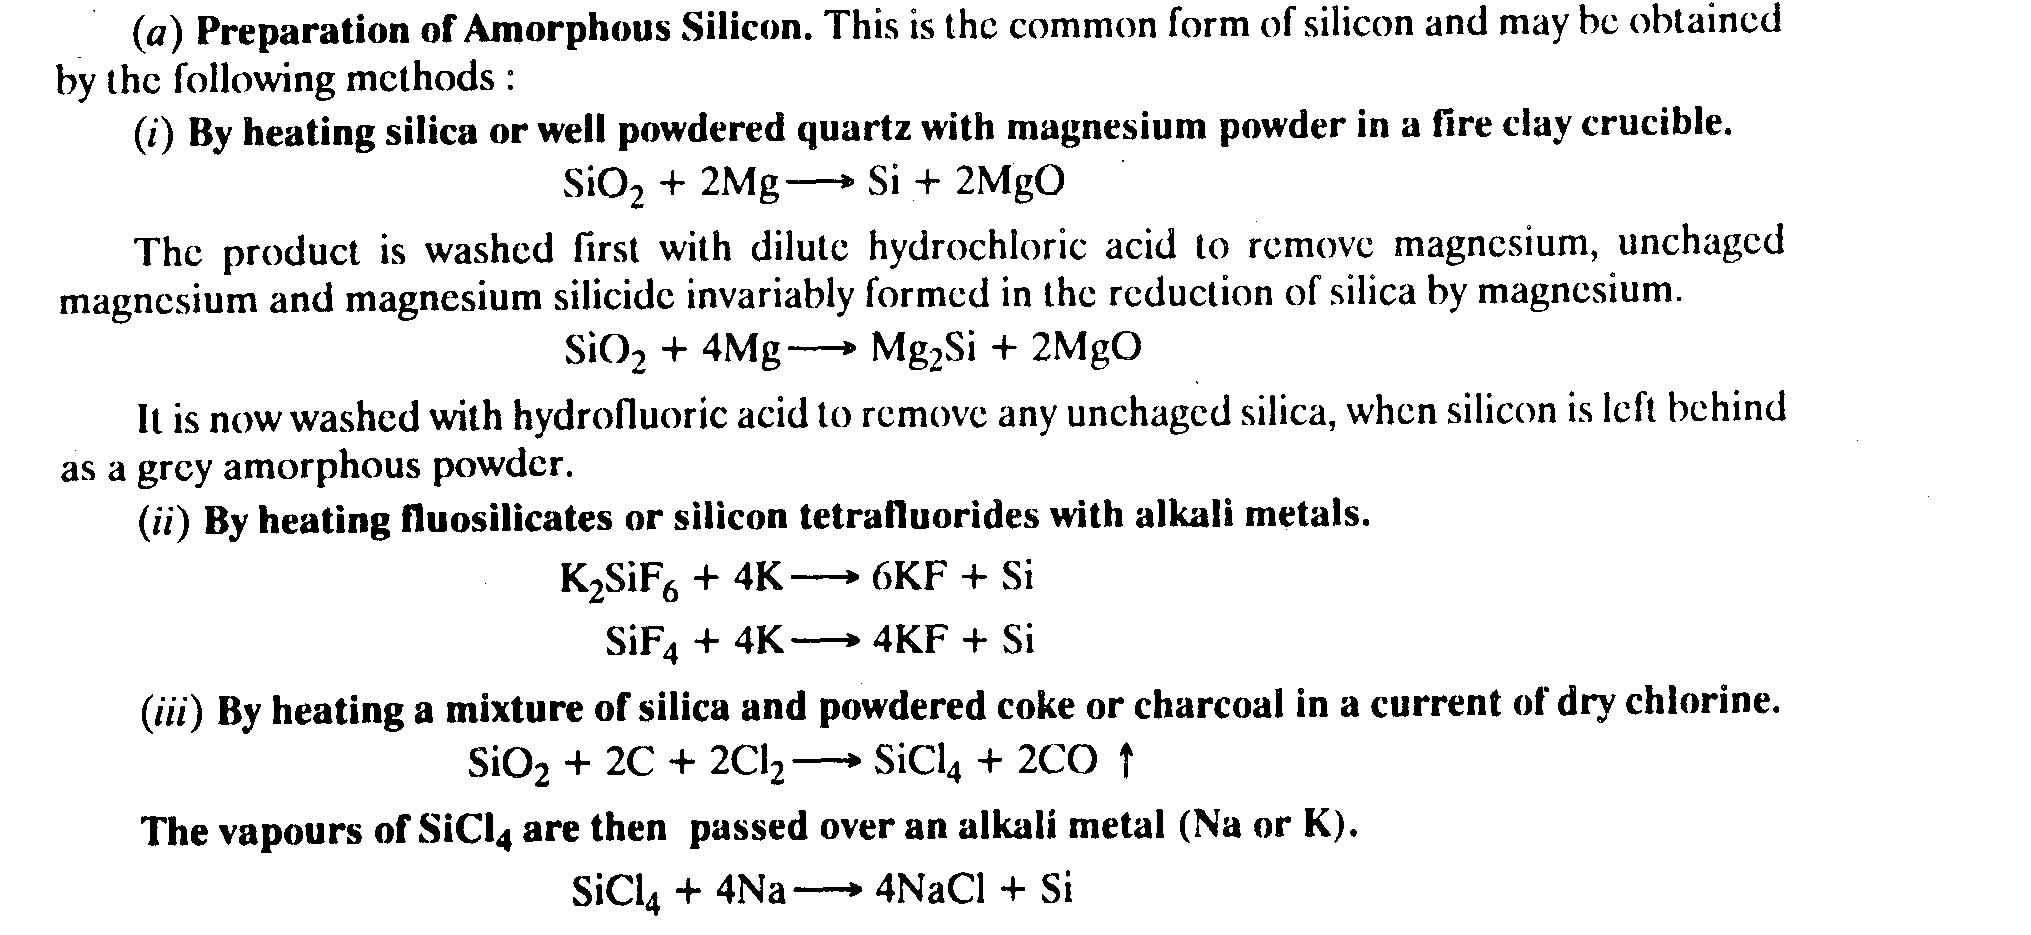
\includegraphics[width=0.3\textwidth]{sampleDocument.png} \\ (a) \\
 \hline
 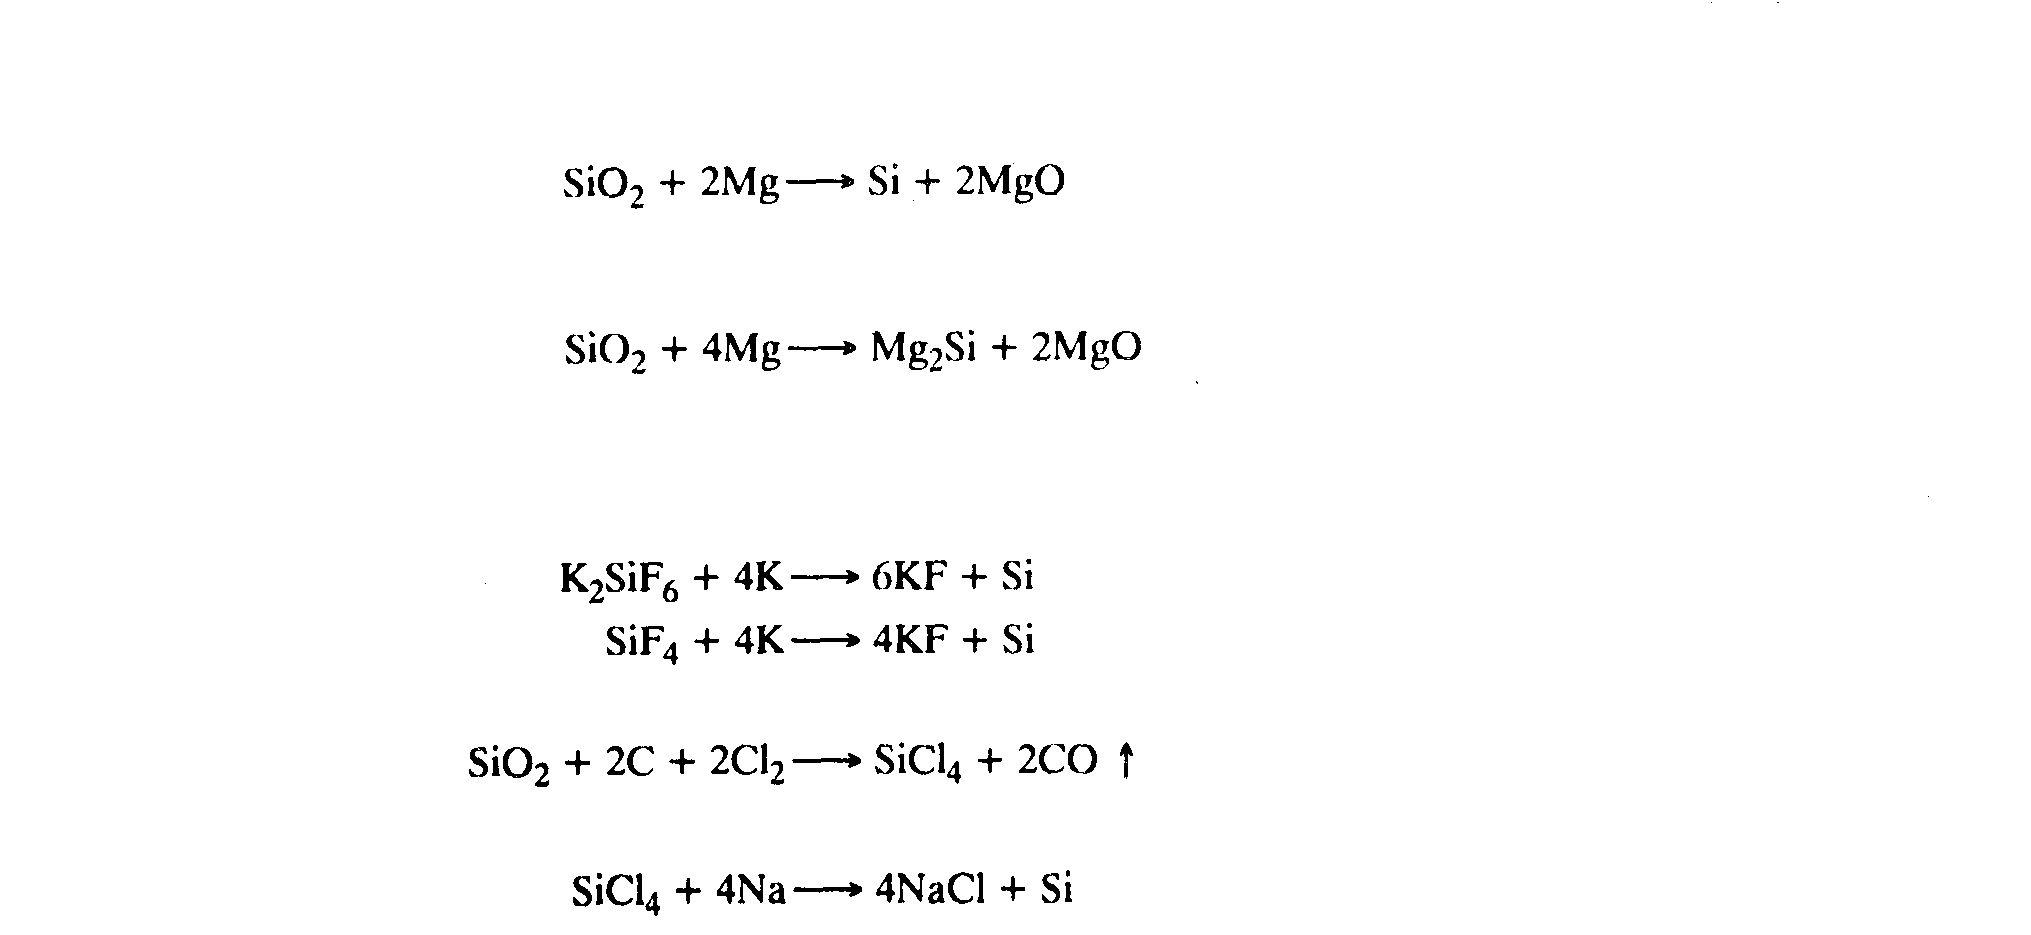
\includegraphics[width=0.3\textwidth]{DCE.png} \\ (b) \\ 
%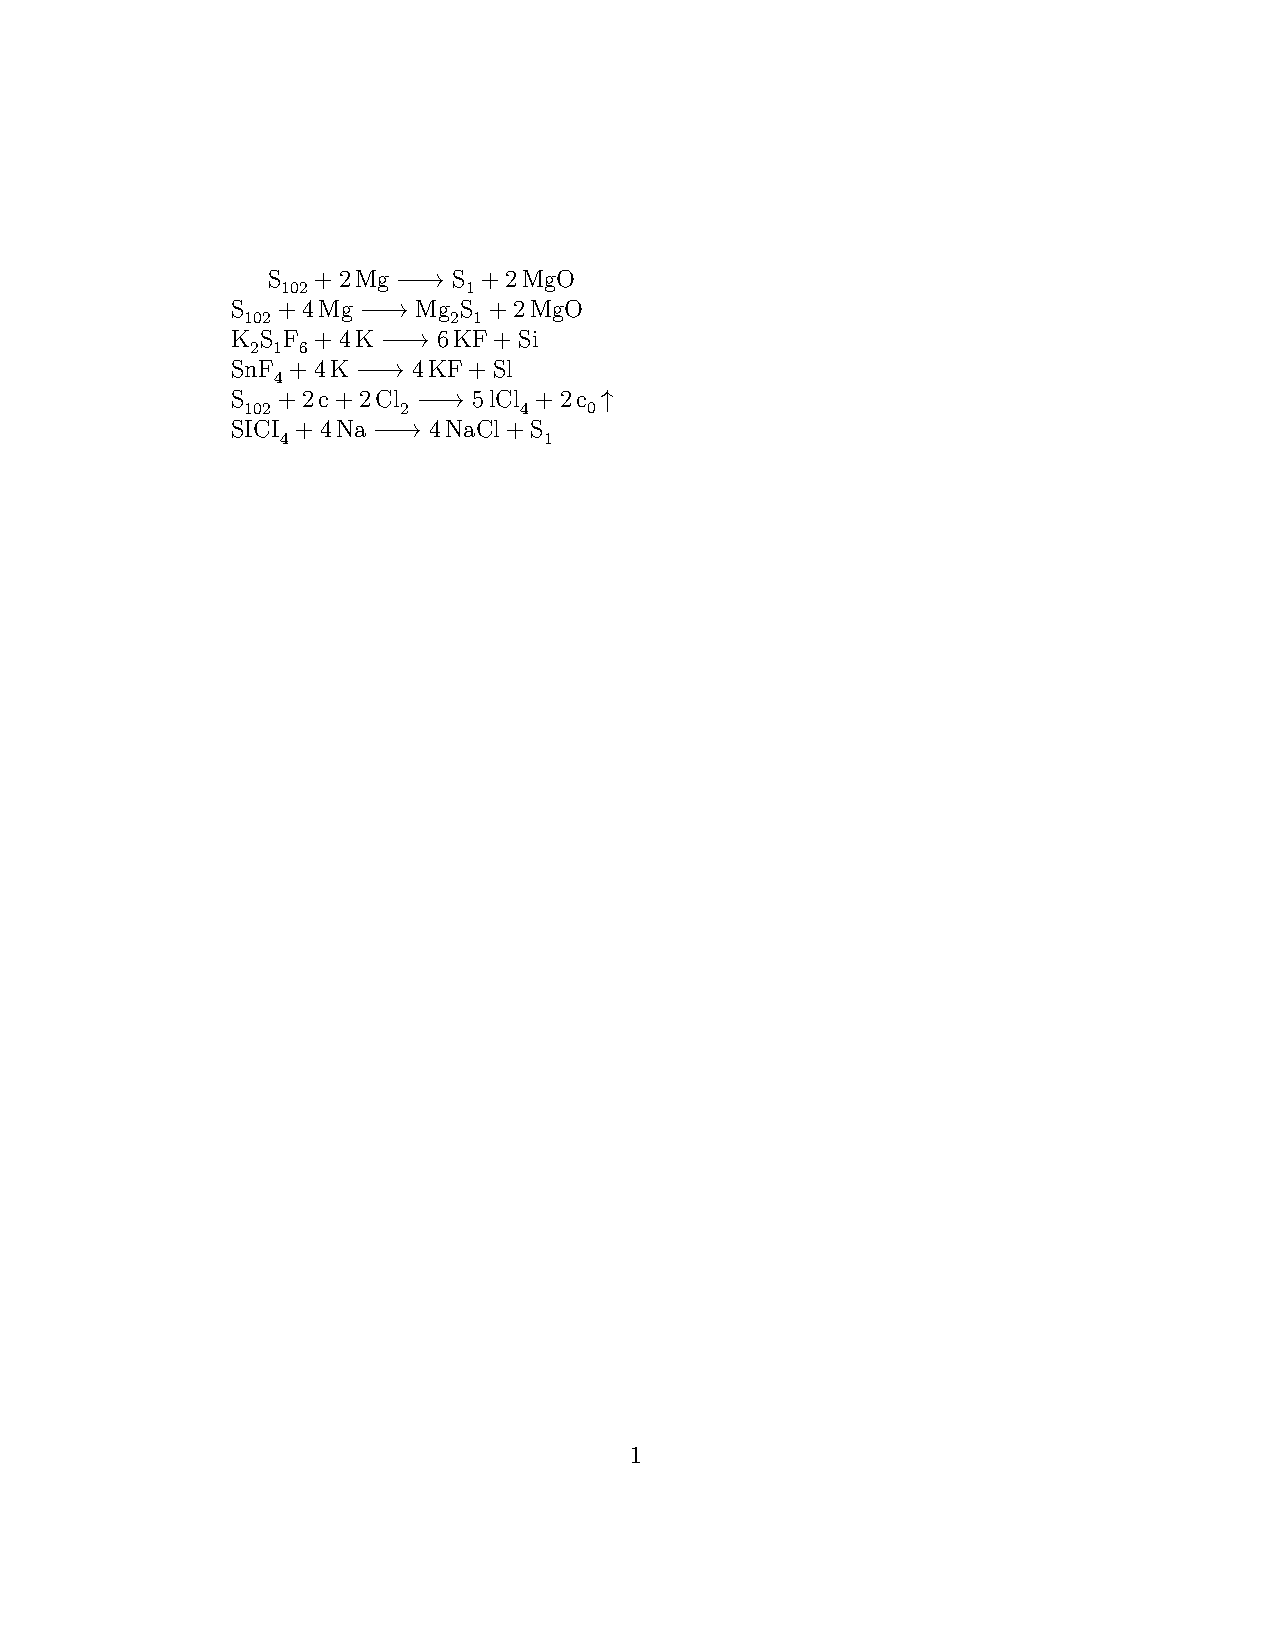
\includepdf[(pages={1})]{ directOCR.pdf } \\
\hline
 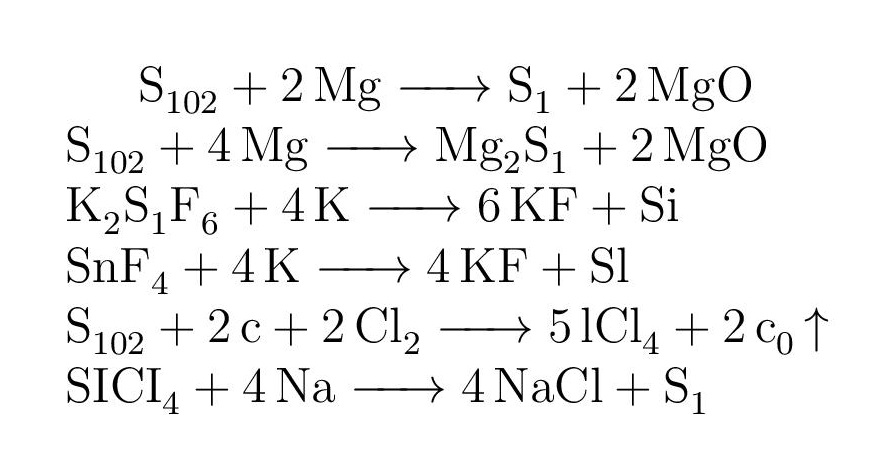
\includegraphics[width=0.3\textwidth]{directOCR.jpg} \\
%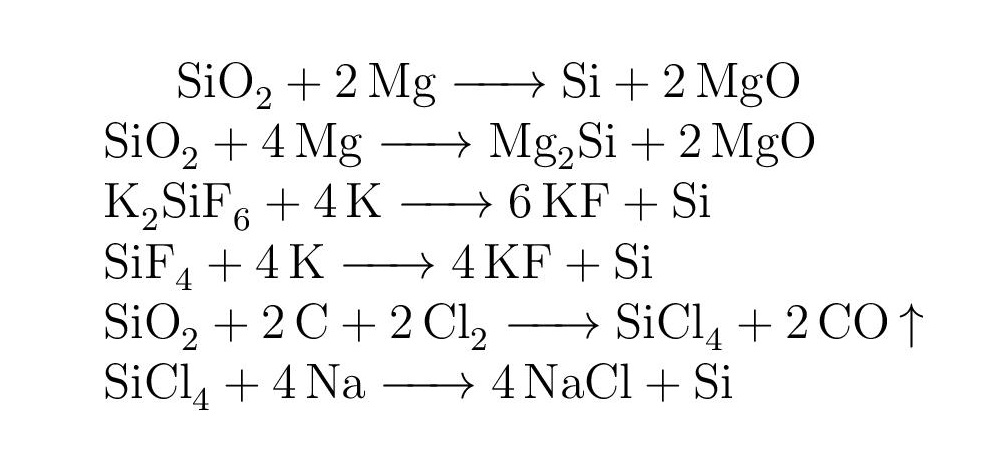
\includegraphics[width=0.25\textwidth]{correctedFinalEq.jpg}\\
 
 (c)  \\
 \hline
\end{tabular}
\caption{Experimental result; (a) Input image; (b) Segmented Chemical equation;
(c) OCR output in PDF format.}%; (d) Output of the proposed method.}
\label{eg} 
\end{figure}


%%%%%%%%%%%%%%%%%%%%%%%%%%%%%%%%%%%%%


\subsection{Refinement of OCR output}
     Due to the limitations of OCR, the output of OCR is not fully correct in the paradigm of  chemical equation/formula. 
      Out of 3406 chemical compounds in our dataset, the accuracy of  OCR conversion  is only 43.13\%. Hence,  refinement of the recognized chemical formula in the equations is  an absolute necessity. 

The output of closing operation is taken as input here. 
Each connected component i.e. character within a word blob is an input to the the OCR and the corresponding output  is stored in a cell and these cells form a string (S$_{chemical}$) for each word blob. For each superscript and subscript, `\^{}'  and  `\_' are inserted before them respectively in S$_{chemical}$.

 First, an error table is created based on the observation of OCR outputs of 280 chemical equations consisting of 1022 compounds (Table~\ref{table:errorTable}).
 Table~\ref{table:errorTable} consists of two columns; first column is actual input to the OCR and the second column contains all erroneous OCR outputs.
  Next, this table is stored into a hash map $H$ where each key is the erroneous OCR output and its value is the possible input set. 
  Table~\ref{table:hashmap} shows this hash map where the first column is the key and the second column contains its corresponding values.
% Auto correction is performed based on this error hash map ($H$).
For example, if `$8$' is an erroneous OCR output for inputs `$g$', `$3$' and `$a$' (Table~\ref{table:errorTable}) then, in the hash map $H$ (Table~\ref{table:hashmap}) , the key is `$8$' and its corresponding value is [$g$, $3$, $a$] .

\begin{table}
\captionof{table}{Part of the Error list}
\begin{center}
 \begin{tabular}{|| c | c ||}
 \hline
 correct input & corresponding erroneous OCR outputs\\
 \hline
 g & 8 3 S\\
 \hline
O & 0\\
\hline
3 & 8 'E s w \\
\hline
a & 3. 21 8 El 8. \\
\hline
l & 1 I\\
\hline
s & S\\
\hline
%\textcolor{red}{expanded} &  \\
 %\hline
n & l1 1'1 I1 11 X1 Il \\
\hline
q & Cl Q\\
\hline
H & 1-l 1-1 l-l l-1\\
\hline
2 & 7 4 Z z\\
\hline
I & l\\
\hline
u & 11 U l1 ll 1l\\
\hline
i & 1 l I\\
\hline
%5 & 'S\\
%\hline
%4 & A\\
%\hline
%Z & 2\\
%\hline
%e & C\\
%\hline
%c & C\\
% \hline
 
 \end{tabular}
 \end{center}
 \label{table:errorTable}
 \end{table}


\begin{table}
\captionof{table}{Part of the Error Hash Map}
\begin{center}
 \begin{tabular}{|| c | c ||}
 \hline
 Erroneous OCR Output & Possible Input Set\\
 \hline
8 & g 3 a\\
\hline
3 & g \\
\hline 
S & g s \\
\hline
0 & O \\
\hline
'E & 3\\
\hline
s & 3\\
\hline 
w & 3\\
\hline
3. & a\\
\hline
21 & a\\
\hline
El & a\\
\hline
8. & a\\
\hline
1 & l i \\
\hline 
I & l i \\
\hline
l1 & n u\\
\hline
1'1 & n\\
\hline
I1 & n\\
\hline
11 & n u\\
\hline
X1 & n\\
\hline
Il & n\\
\hline
Cl & q\\
\hline
%Q & q\\
%\hline
%1-l & H\\
%\hline
%1-1 & H\\
%\hline
%l-l & H\\
%\hline
%l-1 & H\\
%\hline
%7 & 2\\
%\hline
%4 & 2\\
%\hline
%Z & 2\\
%\hline
%z & 2\\
%\hline
%l & I i\\
%\hline
%U & u\\
%\hline
%ll & u\\
%\hline
%1l & u\\
%\hline
%'S & 5\\  
%\hline
%A & 4\\
%\hline
%2 & Z\\
%\hline
%C & e c\\
%\hline 
 \end{tabular}
 \end{center}
 \label{table:hashmap}
 \end{table}

\begin{figure}[h]
\center\ 
\begin{tabular}{|c|} 
\hline
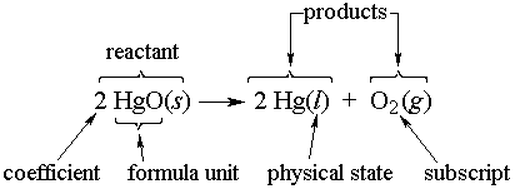
\includegraphics[width=0.3\textwidth]{chemEqParts.png}\\
\hline
\end{tabular} 
\caption{Different components of a chemical equation. }
\label{chemEqParts} 
\end{figure}  

 Each chemical compound in any equation (Fig.~\ref{chemEqParts}) has the following format - 
 
 [Coefficient]$^{[0,1]}$[Formula Unit][State]$^{[0,1]}$. 
 
 This represents that each chemical compound in an equation may or may not start with a numeric Coefficient, must be followed by a \emph{Formula Unit} and may or may not end with a \emph{State} representation. 
    Hence, refinement or auto correction of the OCR output corresponding to each word blob includes the following steps - (i) Coefficient extraction; (ii) State separation; (iii)Auto correction of the formula unit; and (iv) Auto correction of the entire equation using Context Table.


\subsubsection{Coefficient Extraction}
Numeric coefficient denotes the number of molecules/atoms taking part in the reaction. Coefficient extraction is done by matching its regular expression $[2-9]^{+}[0-9]^{*}$ at the beginning of S$_{chemical}$ as it has numerical values. In the regular expression, + indicates number of occurrence must be 1 or greater and * indicates the occurrence is 0 times or greater. 0 and 1 are excluded from the first digit as number of molecules or atoms cannot be 0 and if the number is 1, the numeric coefficient is not mentioned by default. Matched coefficients are stored in S$_{coeff}$. 

\subsubsection{State separation}
 The four physical states of a chemical compound - solid, gaseous, liquid, and aqueous are denoted by `(s)', `(g)', `(l)', and `(aq)', respectively. To detect the physical state of the compound,  regular expression 
   [(][A-Za-z0-9]$^{+}$[)] is used and the checking starts from the end of S$_{chemical}$. The matched substring, $S$ is extracted from  S$_{chemical}$ and Algorithm~\ref{alg:getAllCombs} is run. As mentioned earlier, OCR output for each character is stored in a cell of $S$.
In this algorithm, $S$ (after removing first and last character - opening   and closing brackets) and $H$  are taken as inputs and all possible $Combinations$ of  OCR output is produced by $GetAllCombinations$ (See Fig.~\ref{stateCorrection}). For each cell element in $S$, corresponding values from  hash map, $H$ is assigned to a set, $InputSet$ (See Line 3 in Algorithm~\ref{alg:getAllCombs}). This set contains all possible inputs to the OCR system. 
Now, the key itself is added with its corresponding values in the hash table to make the $InputSet$  if the length of key  is 1. For example, `8' is added to the $InputSet$ as its length is 1 (Fig.~\ref{stateCorrection}). On the contrary, in the second $InputSet$, `Cl' is not included  as its length is 2 (Fig.~\ref{stateCorrection}).


Each cell element of $S$ gives one $InputSet$. Now, cartesian product of all the  $InputSet$ is taken to give us all possible $Combinations$ and only one of the combinations is correct under proper chemical context.
These $Combinations$ are compared with `s', `g', `l' and `aq'. If no match is found, the substring extracted from S$_{chemical}$ is concluded as a radical 
( Fig.~\ref{radical}, the compound contains a radical having the same regular expression mentioned earlier)
, not a state; else, we separate the state from the compound and store it in S$_{state}$ (after adding `(' and `)' at the start and end of $S$). 

\begin{algorithm}
\small
\caption{Attempts to find out all possible combinations of the initial error corrected OCR converted texts}
\begin{algorithmic}[1]
	%\qinput{description of algorithm input}
\Procedure {GetAllCombinations}{$S$,$H$}
	%\State \textbf{Input:} {$CC, H$}
	%\State \textbf{Output:} {$Combinations$}
%	\ForAll {$element(s) \in S$}
%		\State $InputSet \leftarrow H.Get(element)$ 
%		\If {$InputSet$ is $NULL$}
%			\State $RETURN$ \Comment Not in Error Map
%		\Else
%			\If {$length(element) = 1 $}
%				%\State $InputSet =\cup$  $element $
%				\State $InputSet =\cup$ $[element]$ 
%				\Statex \Comment Element might be correct output but still in the error list for other inputs
%			\Else
%				\State \textbf{Ignore}
%				\Statex \Comment Input is one character, output length $>$ 1 means error
%			\EndIf
%		\EndIf
%	\EndFor
%\State $Combinations \leftarrow CartesianProduct(InputSet)$ %\Comment CartProd : Cartesian Product
%\State  \textbf{Return} {$Combinations$}

\State For each element in S, corresponding values from H is assigned to a set, InputSet
\State If the InputSet is null, this indicates that the OCR output is not in the Hash map
\State Since each element is OCR output of one letter, its ideal text length should be 1. Anything more than that indicates error
\State Cartesian product of all letters in InputSet is taken and stored into an 2D array, Combinations

\EndProcedure
\Statex
\end{algorithmic}
\label{alg:getAllCombs}
\end{algorithm}


\begin{figure}[h]
\center\ 
\begin{tabular}{|c|} 
\hline
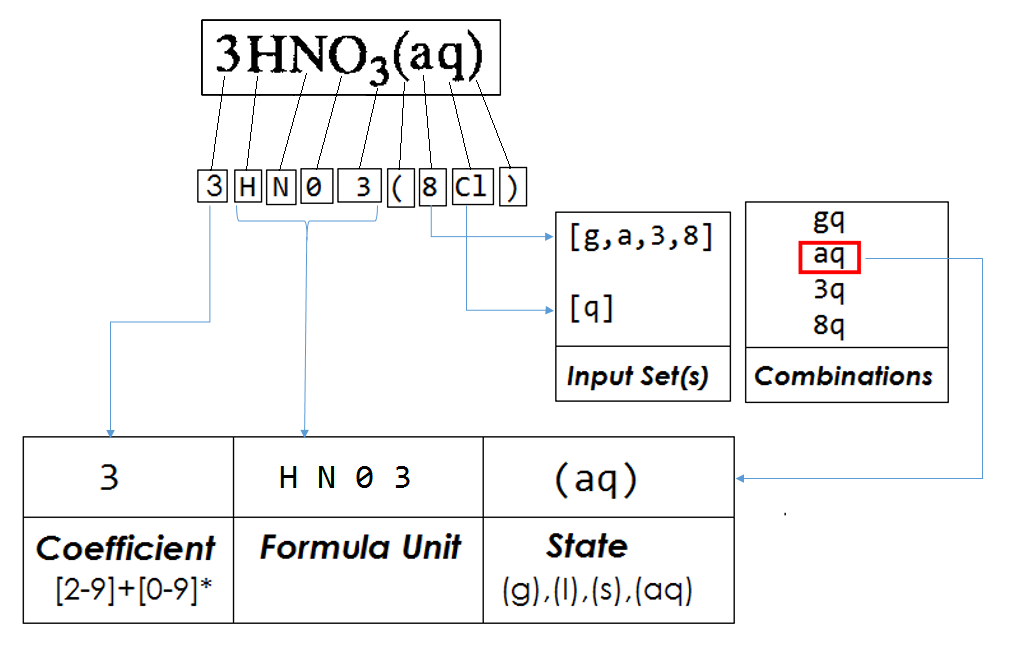
\includegraphics[width=0.3\textwidth]{stateCorrection.png}\\
\hline
\end{tabular} 
\caption{Extracting the formula unit, numeric coefficient and physical state from a chemical compound. }
\label{stateCorrection} 
\end{figure} 

\begin{figure}[h]
\center\ 
\begin{tabular}{|c|} 
\hline
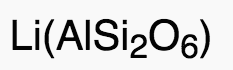
\includegraphics[width=0.25\textwidth]{radical.png}\\
\hline
\end{tabular} 
\caption{Example of chemical compound having a radical in the end. }
\label{radical} 
\end{figure} 



\begin{figure}[h]
\center\ 
\begin{tabular}{|c|c|} 
\hline
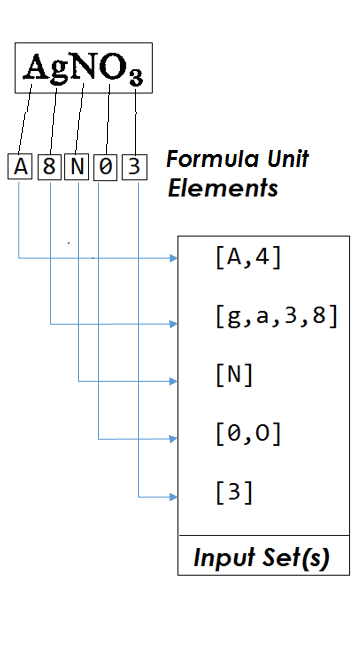
\includegraphics[width=0.12\textwidth]{autoCorrectionPictorial-a.png} &
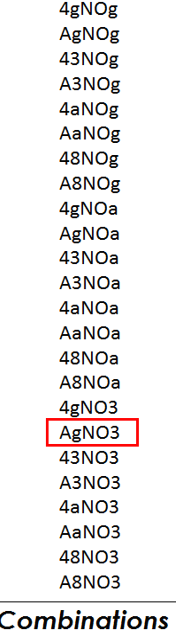
\includegraphics[width=0.12\textwidth]{autoCorrectionPictorial-b.png}\\
(a) & (b) \\
\hline
\end{tabular} 
\caption{Example of auto correction of a formula unit. }
\label{autoCorrection} 
\end{figure} 


\subsubsection{Refinement of the formula unit}
After extracting coefficient and state, only the formula unit is left in S$_{chemical}$. 
The algorithm for auto correction of each formula unit is done in two steps using Algorithm~\ref{alg:getAllCombs} and Algorithm~\ref{alg:findMatch}. First, Algorithm~\ref{alg:getAllCombs} is performed on the formula unit to get all possible combinations. 
 Next, the output of Algorithm~\ref{alg:getAllCombs}($Combinations$) is taken as the input of Algorithm~\ref{alg:findMatch}.  This algorithm is used to match the $Combinations$  against a nearly exhaustive list of all molecules, chemical compounds, radicals and atoms namely $ChemList$ collected from Wikipedia. 
 \footnote{\url{http://en.wikipedia.org/wiki/Dictionary_of_chemical_formulas}}.
 
Three  cases may arise as follows--  

(i) Exactly one match -- \\
 Fig.~\ref{autoCorrection}(b) shows the output of Algorithm~\ref{alg:getAllCombs}. This is matched against $ChemList$ using Algorithm~\ref{alg:findMatch} and algorithm finds one exact match as indicated by the red rectangle. This match is considered as the $Corrected$ formula unit.
 
 (ii) No match -- \\
Longest common substring(s) (LCS) between $Combinations$ and $ChemList$ is computed and the formula unit in $Chemlist$ having the longest common substring with $Combinations$ is considered as  $SubMatch$. There can be multiple such $SubMatch$.
If there is only one, then the corresponding formula unit in $ChemList$ is considered as the $Corrected$  formula unit; else the $SubMatch$es having the same length as that of the $Combinations$ are considered as $PossibleFormulaUnit$s. Fig.~\ref{nabr} (a) is a sample chemical compound. The OCR converted string is `N 21 B l'. Algorithm~\ref{alg:getAllCombs} returns `NaBI' and `NaBl' as the two combinations. None of them match with any chemical compound in $ChemList$. Hence, LCS is computed between these two possible combinations and $ChemList$. Six compounds with LCS length 3 is found as shown in Fig.~\ref{nabr}(b). Since the number of $SubMatch$es is six, the $SubMatch$ having the closest length as that of $Combination$ (i.e. 4) is considered as $PossibleFormulaUnit$. In this case, it is `NaBr'.

\begin{figure}[h]
\center\ 
\begin{tabular}{|c|} 
\hline
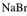
\includegraphics[width=0.1\textwidth]{nabr.png} \\ (a) \\ \hline
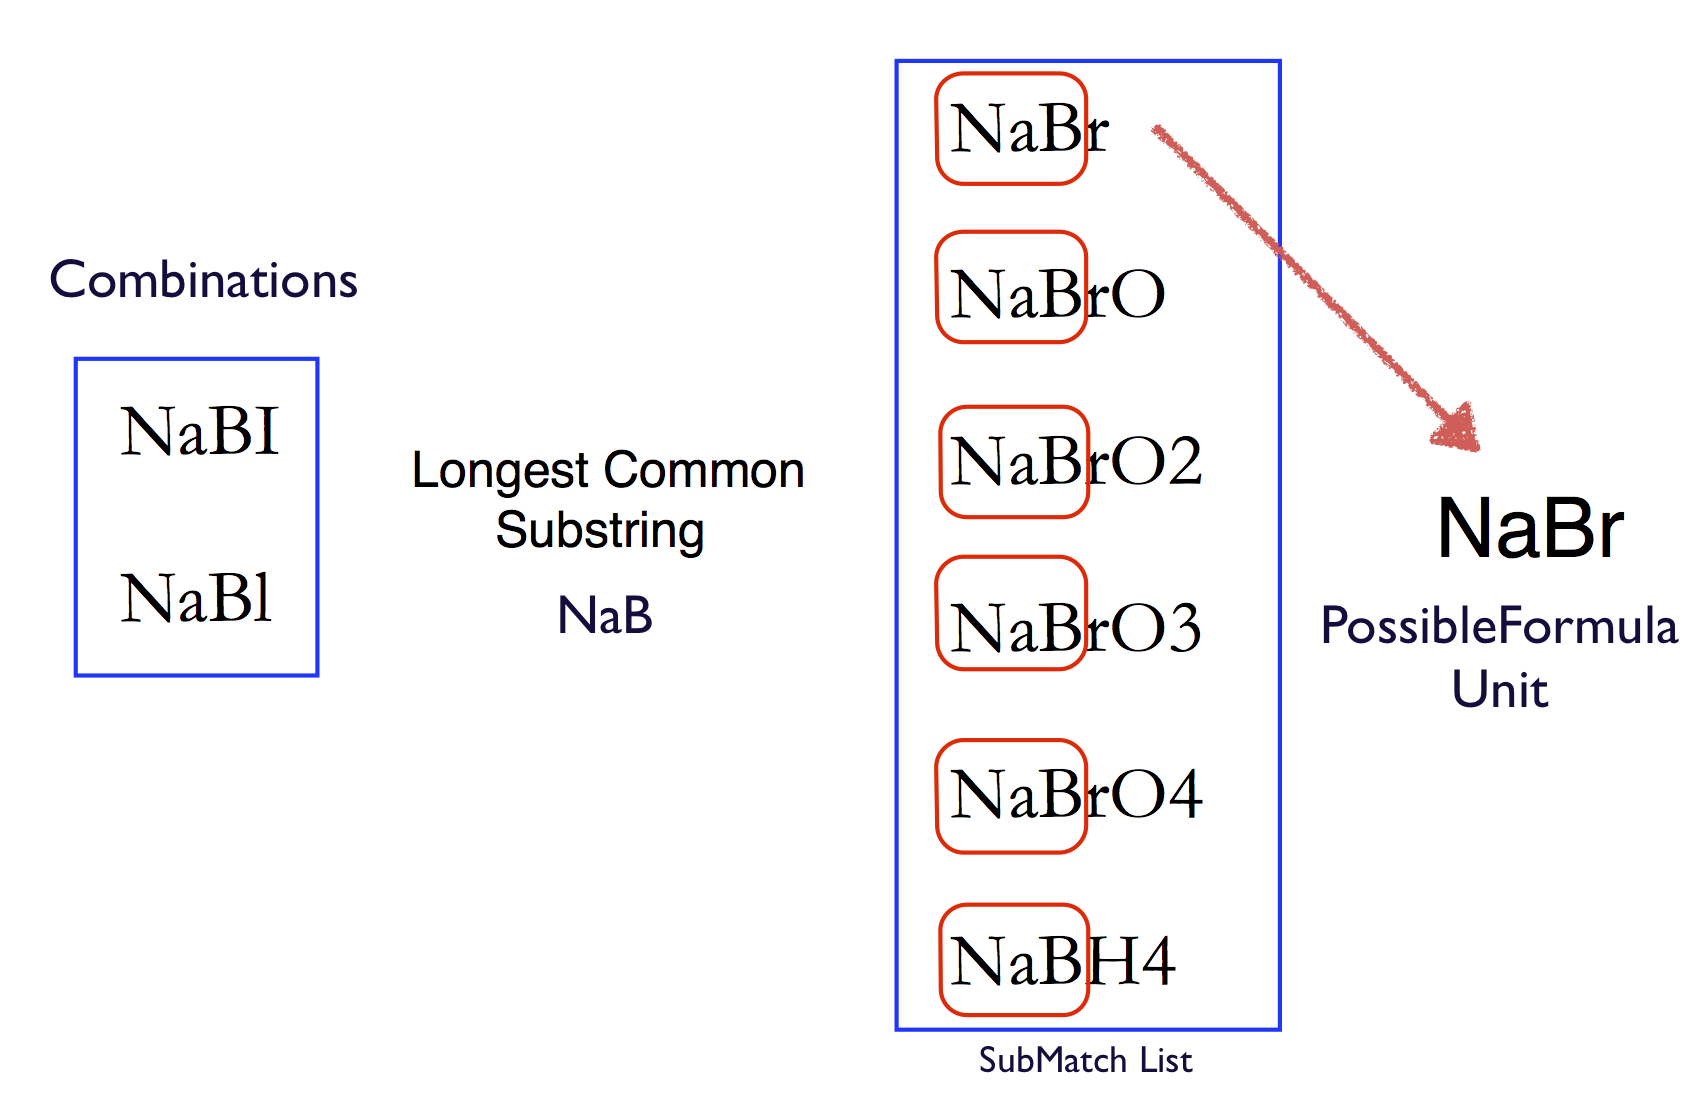
\includegraphics[width=0.3\textwidth]{lcs.png} \\ (b) \\
\hline
\end{tabular} 
\caption{(a) Sample Chemical Compound; (b) LCS Match. }
\label{nabr} 
\end{figure} 
%\item

(iii) More than one exact match -- \\ In Fig.~\ref{context}, `u' of `Cu' in left hand side of the equation is  `l1' as the output of OCR. Among all possible combinations returned by Algorithm~\ref{alg:getAllCombs}, `Cu' and `Cn' both match with $ChemList$. Hence, more than one exact match are found and  both are considered as $PossibleFormulaUnit$.

The above steps are precisely mentioned in Algorithm~\ref{alg:findMatch}. This algorithm returns $Corrected$ and \\$PossibleFormulaUnit$s upon which context analysis is done and is discussed in the next section.  

\begin{algorithm}
\small
\caption{Find Match between ChemList and Combinations derived from Algorithm~\ref{alg:getAllCombs}}
\begin{algorithmic}[1]
\Procedure {FindMatch}{$ChemList$,$Combinations$} %\Comment $ChemList$ : nearly exhaustive list of all molecules and chemical compounds
%	\ForAll{$Combinations$}
%		\State \textbf{match} {with $ChemList$}
%	\EndFor
%	\If {\#(Match Found) = 1}
%		\State $Corrected \leftarrow Match$
%		\State  \textbf{Return} {$Corrected$}
%	\ElsIf {\#(Match Found) = 0}
%		\State $SubMatch \leftarrow \textbf{LCS match}(Combinations,ChemList)$ 
%		\Statex \Comment LCS : Longest Common Substring
%		\If {\#($SubMatch$)=1}
%			\State $Corrected \leftarrow SubMatch$
%			\State  \textbf{Return} {$Corrected$}
%		\Else
%			\State $PossibleFormulaUnit(s) \leftarrow SubMatches$
%			\Statex having closest length as $Combination$
%			\State  \textbf{Return} {$PossibleFormulaUnit(s)$}
%		\EndIf
%	\Else
%		\State $PossibleFormulaUnits \leftarrow Matches$
%		\State  \textbf{Return} {$PossibleFormulaUnit(s)$}
%		\Statex \Comment Multiple matches
%	\EndIf

\State Each combination is looked up against ChemList to find a match. Depending on the type of match, different steps are taken
\State If it's an exact match, that combination is considered as Corrected compound
\State If it's not an exact match, longest common substring of that combination and ChemList is taken. If there are multiple longest common substrings, all of them are considered for next steps
	\If {The longest common substring is a match with ChemList\\}
	 \State This is considered as Corrected compound
	\Else
	\State The longest common substring(s) is(are) stored as PossibleFormulaUnit(s)
	\EndIf

\EndProcedure
\end{algorithmic}
\label{alg:findMatch}
\end{algorithm}

%%%%%%%%%%%%%%%%%%%%%%%%%%%%%%%
%%%%%%%%%%%%%%%%%%%%%%%%%%%%%%%
%%%%%%%%%%%%%%%%%%%%%%%%%%%%%%%


\subsubsection{Auto correction of the entire equation using Context Table}
Here, we have $Corrected$ and $PossibleFormulaUnit$(s) and try to find out the $FinalEquation$ in the context of the equation itself. If a chemical equation does not have any $PossibleFormulaUnit$, context analysis is not required. The process exits after performing Line 2 of Algorithm~\ref{alg:alg3}.

\begin{figure}[h]
\center\ 
\begin{tabular}{|c|} 
\hline
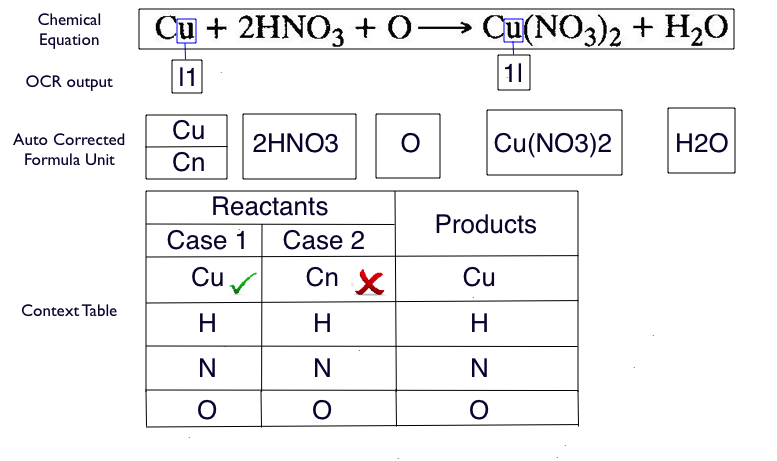
\includegraphics[width=0.3\textwidth]{equationContext_1.png}\\
\hline
\end{tabular} 
\caption{Formation of context table. }
\label{context} 
\end{figure}


Algorithm~\ref{alg:alg3} takes all $Corrected$ and \\$PossibleFormulaUnit$s and returns the $FinalEquation$ by forming the Context Table. 
As the universe is a closed system, all chemical equations have the same periodic elements in the left hand side, called $Reactants$ as that in the right hand side, called $Products$. All the periodic elements follow the regular expression [A-Z][a-z]*. So, for each  $PossibleFormulaUnit$, the set of periodic elements in the $Reactants$, $P_{R}$ and in the $Products$, $P_{P}$ are computed and stored in the $Context Table$. 
When the set difference of $P_{R}$ and $P_{P}$ in the table is empty, that $PossibleFormulaUnit$ is considered as $Corrected$ (Fig.~\ref{context} Case 1). In the Case 1 of  $P_{P}$, the empty set condition satisfies. Hence, `Cu' will be the $Corrected$ formula unit, not `Cn'. But if the above condition comes true for multiple possibilities, we cannot decide which of the possible formula units are actually in the original equation. This is considered an $ERROR$ case.
%An example of formation of context table is demonstrated in  Fig.~\ref{context}.
 Finally, S$_{coeff}$ and S$_{state}$ ( if any ) are added with their corresponding $Corrected$ formula unit after the context analysis and this results in $FinalCompound$s for each equation. 

Now according to the stoichiometry of the chemical reaction, pre-recognised operators along with $FinalCompound$s are concatenated together. This gives us the final auto-corrected chemical equation.


\begin{algorithm}
\small
\caption{Auto-Correction of the entire equation using chemical context table}
\begin{algorithmic}[1]
\Procedure {GetFinalEqn}{$PossibleFormulaUnit$,$Corrected$}
%	\State {Include all $Corrected$ units in $FinalCompound$}
%	\State{$Count  \leftarrow 0$}
%	\For{every $PossibleFormulaUnit$}
%		\State \textbf{compute}($P_{R}$)  
%		\Statex \Comment{$P_{R}$ :  Set of periodic elements in Reactants}
%		\State \textbf{compute}($P_{P}$)  \
%		\Statex \Comment {$P_{P}$ : Set of periodic elements in Products}
%		
%		\If{$P_{R} - P_{P} = \emptyset $}
%			\State $Corrected \leftarrow PossibleFormulaUnit$
%			%\State {Include that in the $FinalEquation$}
%			\State $Count \leftarrow Count + 1$
%		\EndIf
%	\EndFor
%	\If {$Count = 1 $}
%		\State { $FinalCompound \leftarrow [S_{coeff}, Corrected, S_{state}] $ }
%	\ElsIf {$Count = 0 $}
%		\State Break
%	\Else 
%		\State {Multiple $Corrected$ compounds}
%		%\State{Multiple $FinalEquations$}
%		\Statex \Comment { $ERROR$}
%	\EndIf
%	\State  \textbf{Return} {$FinalCompund(s)$}
	
\State All PossibleFormulaUnits and Corrected compounds from Algorithm 2 are taken as input and all corrected compounds are directly placed in the equation 
\State Now for every PossibleFormulaUnits in the Reactants side, set of periodic elements are computed (Pr)
\State Similarly for every PossibleFormulaUnits in the Products side, set of periodic elements are computed (Pp)
\State If Pr and Pp are complete match, then that PossibleFormulaUnit is taken as Corrected and placed into the final equation
\State Now finally with every corrected compound corresponding coefficient and state is added before and appended respectively
\State If there are multiple Corrected compounds for one PossibleFormulaUnit then this algorithm  fails and shows all possible corrected final equations

	
\EndProcedure
\end{algorithmic}
\label{alg:alg3}
\end{algorithm}





%%%%%%%%%%%%%%%%%%%%%%%%%%%%%%%%%%%%%%%



\subsection{Generation of chemical equation in search-able PDF format} 
\label{mhchem}
The final auto-corrected chemical equation
 is then converted to \LaTeX\  using the format specified by $mhchem$ 
  \footnote{\url{ftp://www.ctan.org/tex-archive/macros/latex/contrib/mhchem/mhchem.pdf}}
 package which provides commands or typesetting chemical molecular formulae and equations. This produces the searchable PDF format. 


\section{Experimental Result}
\label{sc:exp}
We have implemented our algorithm in MATLAB 8.3.0.532
(R2014a) in a PC (Intel(R) Core(TM) i5-3337U CPU @ 1.80GHz
running Windows 8). The proposed method has been tested on
a dataset consisting of 234 document images. Out of 234 pages 50 are taken from ICDAR 2013 Math-zone segmentation datasets and other document pages are scanned from different Mathematics and
Chemistry books. 
The summary of the experimental results
is shown in Table~\ref{table:result}. Out of 3406 chemical formula in the test dataset, 114 formula were partially corrected and 52 formula could not be corrected at all. The overall accuracy of complete refinement  is 95.12\%. This is measured by (\#Completely Corrected formula / \#Total number of formula). Due to the longest common substring match and then performing context analysis of the entire equation, there is a very small window of zero correction. 
Zero correction is the case when there have been no correction to the OCR output by the auto-correction algorithm. For example, OCR output of `Mg'- $I^I3$ could not be corrected by our auto-correction algorithm as this erroneous conversion was not in the error hash map.



With our dataset, zero correction rate is 0.01\% (It is computed as \#Zero Correction Compound / \#Total Compounds).These results are quite encouraging. 

Consider the sample image (Fig.~\ref{eg}(a)) and its corresponding segmented displayed chemical equations are shown in Fig.~\ref{eg}(b). Fig.~\ref{eg}(c) shows the direct OCR output where `i' has been wrongly identified as `l', `I' and `1' (for $Si$ in all the lines of  Fig.~\ref{eg}(c)). Similarly `O' results in `0' (line 1,2,3). `S' sometimes is detected as `5' (line 5). Our auto correction algorithm remedies these issues. Fig.~\ref{fin} demonstrates the effect of our auto correction algorithm. This algorithm is targeted towards chemical equation with linear representation. Organic bonds cannot be detected in this system.

Some sample experimental results are shown in Fig.~\ref{sample1}, Fig.~\ref{sample2}, Fig.~\ref{sample3} and Fig.~\ref{sample4}. More results are shown in \url{https://sites.google.com/site/chemeqndb/home}.

\begin{figure}[h]
\center\ 
\begin{tabular}{|c|} 
\hline
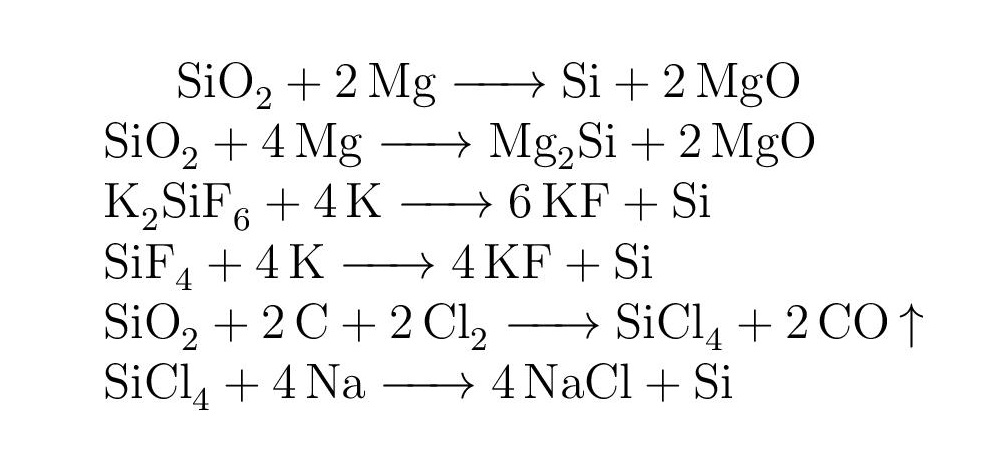
\includegraphics[width=0.3\textwidth]{correctedFinalEq.jpg}\\
\hline
\end{tabular} 
\caption{Auto corrected output of Fig.~\ref{eg}(c). }
\label{fin} 
\end{figure}
%%%%%%%%%%%

\begin{table}
\captionof{table}{Summary of Experimental Results}
\begin{center}
 \begin{tabular}{| c | c |}
 \hline
 \#Total Images & 234\\
 \hline
 \#Total DEs & 1390\\
 \hline
Operator recognition & 99.8\% \\
\hline
 DE segmentation accuracy & 98.63\% \\
 \hline
Chemical DE Classification Accuracy & 98.83\%\\
\hline 
\#Total Chemical Operands & 3406\\
\hline 
Complete refinement accuracy & 95.12\% \\
\hline
Zero Auto correction rate & 0.01\% \\
\hline

 \end{tabular}
 \end{center}
 \label{table:result}
 \end{table}



Next, we try to analyse the sources of some of the errors and shortcomings of our algorithm which have negative effect on the performance figures for auto correction. 

\emph{Case 1} : Chemical equations sometimes contain some texts such as `$and$', `$or$' etc between two chemical compounds (See Fig.~\ref{error}(a)). Sometimes two chemical equations are conjuncted by these words in the same line. If these words are not in chemical context and OCR does not convert them correctly, our autocorrection algorithm cannot match them against $ChemList$, hence the error occurs. But OCR conversion has a high accuracy rate for such type of texts. Therefore, this is not a severe error.

\emph{Case 2} : When the chemical compound is written in formats such as $(Na_2SiO_3)_n$ (Fig.~\ref{error}(a)), only $Na_2SiO_3$ is detected based on $ChemList$ and LCS matching. This is considered as a partial autocorrection case.

\emph{Case 3} : Some equations have conditions (pressure, temperature) written over the arrows (See Fig.~\ref{error}(b)). In this work, we only concentrated on chemical compounds in the equation. This does not effect the autocorrection accuracy rate as most of the time they get segmented in separate text lines; else we ignore the over arrow conditions beforehand. 

\emph{Case 4} : Fractions in the numeric coefficients (Fig.~\ref{error}(c)) are not dealt with in our autocorrection algorithm as they are not very common in chemical equations. 

\begin{figure}[h]
\center\footnotesize 
\begin{tabular}{|c|}
\hline
 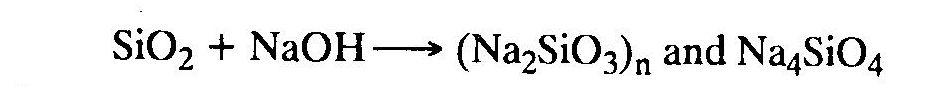
\includegraphics[width=0.3\textwidth]{n.jpg} \\ (a)\\  
 \hline
 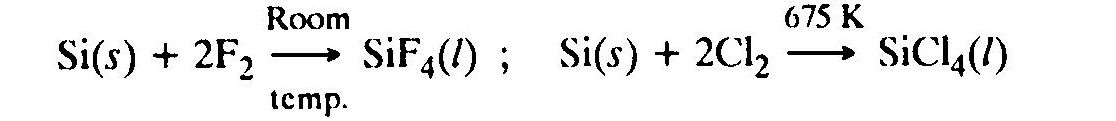
\includegraphics[width=0.3\textwidth]{up.jpg} \\ (b)\\  
 \hline
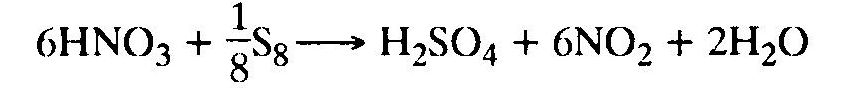
\includegraphics[width=0.3\textwidth]{fraction.jpg} \\ (c) \\ 
\hline
\end{tabular}
\caption{Sample error cases (a) presence of non-chemical words in segmented chemical equation; (b) presence of over arrow conditions; (c) fractional coefficient.}
\label{error} 
\end{figure} 


\emph{Case 5} : Here, in the equation shown in Fig.~\ref{error5}. both the `g's in reactant and product side have been converted to `S'  by the OCR which results in multiple auto-corrected formula units on both side. At this point, we reach Step 17 of  Algorithm~\ref{alg:alg3}  where context table formation cannot conclude which one is the final corrected compound. However, normally the probability of occurrence of such situation is extremely rare, so no further steps are taken to rectify this.

\begin{figure}[h]
\center\ 
\begin{tabular}{|c|} 
\hline
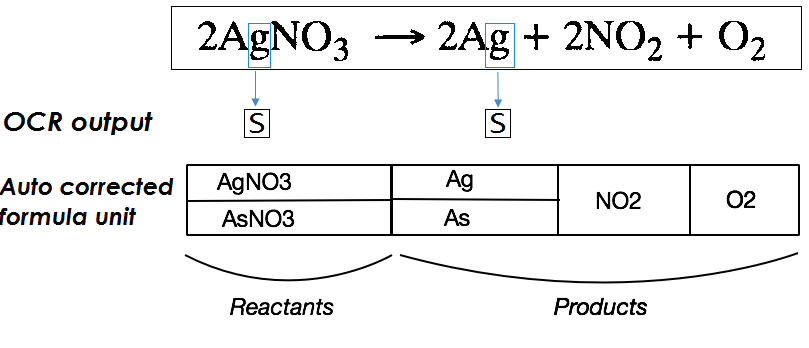
\includegraphics[width=0.3\textwidth]{error5.png}\\
\hline
\end{tabular} 
\caption{ Error case of multiple $Corrected$ compounds}
\label{error5} 
\end{figure}

 
%\begin{figure*}[h]
%\center\ 
%\begin{tabular}{|c|c|} 
%\hline
%\includegraphics[width=0.5\textwidth]{5.jpg} &
%\includegraphics[width=0.5\textwidth]{5copy.png}\\
%(a) Input Image & (b) Segmented Displayed Chemical Equations\\
%\hline
%\includegraphics[width=0.5\textwidth]{5directOCR.pdf} &
%\includegraphics[width=0.5\textwidth]{finalResult_5.pdf}\\
%(c) Direct OCR output & (d) Auto-corrected OCR output\\
%\hline
%\end{tabular} 
%\caption{Experimental result: Sample 1. }
%\label{sample1} 
%\end{figure*}



%\begin{figure*}[h]
%\center\ 
%\begin{tabular}{|c|c|} 
%\hline
%\includegraphics[width=0.5\textwidth]{6.jpg} &
%\includegraphics[width=0.5\textwidth]{6copy.png}\\
%(a) Input Image & (b) Segmented Displayed Chemical Equations\\
%\hline
%\includegraphics[width=0.5\textwidth]{6directOCR.pdf} &
%\includegraphics[width=0.5\textwidth]{finalResult_6.pdf}\\
%(c) Direct OCR output & (d) Auto-corrected OCR output\\
%\hline
%\end{tabular} 
%\caption{Experimental result: Sample 2. }
%\label{sample2} 
%\end{figure*}




\begin{figure*}[h]
\center\ 
\begin{tabular}{|c|c|} 
\hline
\includegraphics[width=0.5\textwidth]{11.jpg} &
\includegraphics[width=0.5\textwidth]{11copy.png}\\
(a) Input Image & (b) Segmented Displayed Chemical Equations\\
\hline
\includegraphics[width=0.5\textwidth]{11directOCR.pdf} &
\includegraphics[width=0.5\textwidth]{finalResult_11.pdf}\\
(c) Direct OCR output & (d) Auto-corrected OCR output\\
\hline
\end{tabular} 
\caption{Experimental result }
\label{sample3} 
\end{figure*}

%\begin{figure*}[h]
%\center\ 
%\begin{tabular}{|c|c|} 
%\hline
%\includegraphics[width=0.5\textwidth]{23.jpg} &
%\includegraphics[width=0.5\textwidth]{23copy.png}\\
%(a) Input Image & (b) Segmented Displayed Chemical Equations\\
%\hline
%\includegraphics[width=0.5\textwidth]{23directOCR.pdf} &
%\includegraphics[width=0.5\textwidth]{23finalResult.pdf}\\
%(c) Direct OCR output & (d) Auto-corrected OCR output\\
%\hline
%\end{tabular} 
%\caption{Experimental result: Sample 4.}
%\label{sample4} 
%\end{figure*}

%
%%%%%%%%%%%%%%%%%%%%%%%%%%%%%%%%%%%%%%%%%





\section{Conclusions}
\label{sc:con}
We have presented an automated chemical equation segmentation and chemical context based auto correction system that is able to provide the exact searchable format of linear chemical equations in any document image. The experimental results demonstrate the efficiency of our proposed method. One of the drawbacks of our system is the time complexity as the search space in the $ChemList$ is quite big and is growing over time due to discovery of new compounds. The search method can be improved and made more efficient. Since our proposed method is novel, we have not concentrated on making the system time efficient yet but more on the accuracy of the auto correction. This work leads to several research avenues. Chemical context horizon can be widened. Auto correction on non-linear or bond structure representations of chemical equations could be ventured in. 





\begin{thebibliography}{1}


\bibitem{blostein_97}
 D. Blostein and A. Grabavec.
\newblock {\em ``Recognition of Mathematical Notation'',}
\newblock {\em Handbook of Character Recognition and document Image Analysis}, 557--582, 1997.

\bibitem{chan_2000}
K-F. Chan and D-Y. Yeung.
\newblock {\em``Mathematical Expression Recognition: A Survey''.}
\newblock {\em IJDAR, Vol. 3, no, 1}, 3--15, 2000.

\bibitem{Garain_07}
U. Garain and B. B. Chaudhuri.
\newblock {\em On OCR of Printed mathematical Expressions.}
\newblock {\em ``Digital Document Processing'',Ed. B. B. Chaudhuri, Advances in pattern 
Recognition}, 235--259 , 2007.

\bibitem{fateman_96}
\newblock R. Fateman, T. Tokuyasu, B. Berman, and N. Mitchell.
\newblock {\em ``Optical character recognition and parsing of typeset mathematics'',
Visual Commun. And Image Representation, Vol 7, no 1}, 2--15, 1996.

\bibitem{toumit_99}
\newblock J. Y. Toumit, S. Garcia-Salicetti, and H. Emptoz.
\newblock {\em ``A hierarchical and recursive model of mathematical expressions for
automatic reading of mathematical documents''. In Proc. of
ICDAR}, 116--122, 1999.
 
\bibitem{kacem_01}
\newblock A. Kacem, A. Beliad and M. Ben Ahmed.
\newblock {\em ``Automated Extraction of printed mathematical formulas using fuzzy logic
and propagation of context'', IJDAR, vol.4 no. 2}, 97--108, 2001.

\bibitem{suzuki_03}
\newblock M. Suzuki, F. Tamari, R. Fukuda, S. Uchida and T. Kanahori.
\newblock {\em ``INFTY - An Integrated OCR system for Mathematical Documents'', Proc. of 
ACM Symposium on Document Engineering}, 95--104, 2003.

\bibitem{Garain_09}
\newblock Utpal Garain.
\newblock {\em `` Identification of Mathematical Expressions in Document Images'',
Proc. of ICDAR}, 1340--1344, 2009.

\bibitem{Garain_05}
\newblock Utpal Garain.
\newblock {\em ``Recognition of Printed Handwritten Mathematical Expressions'', Ph.D Thesis,
ISI, Kolkata, India}, 2005.

\bibitem{Garain_01}
\newblock B. B. Chaudhuri and U. Garain.
\newblock {\em ``Extraction of type atyle based meta-information from Imaged
documents'', IJDAR, vol. 3 no. 3}, 138--149, 2001.

\bibitem{jin_03}
\newblock J. Jin, X. Han and Q. Wang.
\newblock {\em ``Mathematical formulas extraction'', Proc. of ICDAR}, 1138--1141, 2003.

\bibitem{drake_05}
\newblock D. M. Drake and H. S. Baird.
\newblock {\em ``Distinguishing mathematical notation from english text
using computational geometry'', Proc. of ICDAR}, 1270--1274, 2005.

\bibitem{guo_07}
\newblock Y.-S. Guo, L. Huang and C.-P. Liu.
\newblock {\em ``A new approach for understanding of structure of printed mathematical
expressions'', Proc. of ICMLC}, 2633--2638, 2007.

\bibitem{liu_13}
\newblock We-Te Chu and Fan liu.
\newblock {\em ``Mathematical formula detection from heterogeneous document
Images'', Proc. of CTAAI}, 140--146, 2013.

\bibitem{skm_07}
S. P. Chowdhury, S. Mandal, A. K. Das, and B. Chanda.
\newblock {\em ``Segmentation of Text and Graphics from Document Images''},
\newblock in {\em Proc. of ICDAR}, 619--623, 2007.


\bibitem{sekhar_06} S.~Mandal, S.~P.~Chowdhury, A.~K.~Das, and
B.~Chanda, \emph{A simple and effective table detection system
from Document Images}, IJDAR, Vol. 8(2), 172–182, 2006.

\bibitem{spc_07} S.~P.~Chowdhury, S.~Mandal, A.~K.~Das, and
B.~Chanda, \emph{Segmentation of Text and Graphics from Document
Images}, In Proc. of ICDAR, pp. 619–623,2007.

\bibitem{gonzalez92}
R.~C.~Gonzalez and R.~Wood,
\emph{Digital Image Processing},
 Addision-Wesley, 1992.

\bibitem{blostein_97} D.~Blostein and A.~Grabavec,
\emph{Recognition of Mathematical Notation}, Handbook of
Character Recognition and document Image Analysis, 577--582,
1997.
 
\bibitem{chan_00} K-F.~Chan and D-Y.~Yeung, \emph{Mathematical
Expression Recognition: A Survey}, IJDAR, Vol. 3, no: 1, 3–15,
2000.

\bibitem{Garain_07} U.~Garain and B.~B.~Chaudhuri \emph{An OCR
of Printed mathematical Expressions, Digital Document
Processing}, Ed: B.~B.~Chaudhuri, Advances in pattern
Recognition, 235–259 , 2007.

\bibitem{uchid_10}
A.~Fujiyoshi, M.~Suzuki, S.~Uchid,
 \emph{Grammatical Verification for Mathematical Formula Recognition Based on Context-Free Tree Grammar},
 Mathematics in Computer Science, 279--298, 2010.
 
 
 \bibitem{algorri_07}
 M.~E.~Algorri, M.~Zimmermann, C.~M.~Friedrich, S.~Akle, and M.~Hofmann-Apitius,
\emph{Reconstruction of chemical molecules from images},
In Proc. 29th Annual International IEEE Conference on Engineering in
Medicine and Biology Society, 4609--4612, 2007.

\bibitem{algorri_07a}
M.~E.~Algorri, M.~Zimmermann, and M.~Hofmann-Apitius,
\emph{Automatic recognition of chemical images},
In pro. Eighth Mexican International Conference on Current Trends in Computer Science, 41--46, 2007.
\bibitem{park_09}
J.~Park, G.~R.~Rosania, K.~A.~Shedden, M.~Nguyen, N.~Lyu, and K.~Saitou,
\emph{Automated extraction of chemical structure information from digital raster images}, Chemistry Central journal, vol. 3(1), 2009.

\bibitem{nn_tutorial}
A.~K.~Jain, J,~Mao, K.~M.~Mohiuddin
\emph{Artificial Neural Network: A Tutorial}, Computer  (Volume:29 ,  Issue: 3 ), Mar 1996.


\bibitem{prerana_anubhab_15}
 P. Jana and A. Majumdar
\newblock {\em ``Automated Segmentation and Classification of
Chemical and other Equations from Document Images'',}
\newblock {\em 8th International Conference on Advances in Pattern Recognition}, 127-129, 2015.


\end{thebibliography}





%
% The following two commands are all you need in the
% initial runs of your .tex file to
% produce the bibliography for the citations in your paper.
%\bibliographystyle{abbrv}
%\bibliography{sigproc}  % sigproc.bib is the name of the Bibliography in this case
% You must have a proper ".bib" file
%  and remember to run:
% latex bibtex latex latex
% to resolve all references
%
% ACM needs 'a single self-contained file'!
%


\end{document}
